\documentclass{article}
\usepackage{iclr2027_conference,times}
\usepackage[T1]{fontenc}
\usepackage[utf8]{inputenc}
\usepackage{amsmath,amssymb,mathtools,graphicx,booktabs,multirow,makecell,microtype}
\usepackage[table]{xcolor}
\usepackage{hyperref}
\usepackage{url}
\usepackage{placeins}
\usepackage{tikz}
\usetikzlibrary{positioning,fit,calc,backgrounds}
\definecolor{linkink}{HTML}{315B73}
\hypersetup{colorlinks=true,linkcolor=linkink,citecolor=linkink,urlcolor=linkink}

% Every number in the paper comes from tables/result_macros.tex, generated by
% tools/make_tables.py from the evaluation JSONs in results/. \R{key} prints
% the value; an unavailable result prints a red TBD instead of a guess.
% AUTO-GENERATED by tools/make_tables.py -- do not edit by hand.
% AUTO-GENERATED by tools/make_tables.py -- do not edit by hand.
\providecommand{\tbd}{\textcolor{red}{\textbf{TBD}}}
\providecommand{\R}[1]{\ifcsname res@#1\endcsname\csname res@#1\endcsname\else\tbd\fi}
\expandafter\def\csname res@zerodce@L0@psnr_rgb\endcsname{18.19}
\expandafter\def\csname res@zerodce@L0@lpips\endcsname{.429}
\expandafter\def\csname res@zerodce@L1@psnr_rgb\endcsname{17.98}
\expandafter\def\csname res@zerodce@L1@lpips\endcsname{.357}
\expandafter\def\csname res@zerodce@L2@psnr_rgb\endcsname{17.37}
\expandafter\def\csname res@zerodce@L2@lpips\endcsname{.259}
\expandafter\def\csname res@zerodce@L3@psnr_rgb\endcsname{14.80}
\expandafter\def\csname res@zerodce@L3@lpips\endcsname{.335}
\expandafter\def\csname res@zerodce@L4@psnr_rgb\endcsname{17.71}
\expandafter\def\csname res@zerodce@L4@lpips\endcsname{.168}
\expandafter\def\csname res@zerodce@L5@psnr_rgb\endcsname{18.00}
\expandafter\def\csname res@zerodce@L5@lpips\endcsname{.312}
\expandafter\def\csname res@sci@L0@psnr_rgb\endcsname{23.48}
\expandafter\def\csname res@sci@L0@lpips\endcsname{.390}
\expandafter\def\csname res@sci@L1@psnr_rgb\endcsname{17.84}
\expandafter\def\csname res@sci@L1@lpips\endcsname{.343}
\expandafter\def\csname res@sci@L2@psnr_rgb\endcsname{17.79}
\expandafter\def\csname res@sci@L2@lpips\endcsname{.282}
\expandafter\def\csname res@sci@L3@psnr_rgb\endcsname{14.78}
\expandafter\def\csname res@sci@L3@lpips\endcsname{.339}
\expandafter\def\csname res@sci@L4@psnr_rgb\endcsname{15.43}
\expandafter\def\csname res@sci@L4@lpips\endcsname{.233}
\expandafter\def\csname res@sci@L5@psnr_rgb\endcsname{17.30}
\expandafter\def\csname res@sci@L5@lpips\endcsname{.307}
\expandafter\def\csname res@hvicidnet@L0@psnr_rgb\endcsname{19.54}
\expandafter\def\csname res@hvicidnet@L0@lpips\endcsname{.405}
\expandafter\def\csname res@hvicidnet@L1@psnr_rgb\endcsname{18.51}
\expandafter\def\csname res@hvicidnet@L1@lpips\endcsname{.306}
\expandafter\def\csname res@hvicidnet@L2@psnr_rgb\endcsname{18.92}
\expandafter\def\csname res@hvicidnet@L2@lpips\endcsname{.190}
\expandafter\def\csname res@hvicidnet@L3@psnr_rgb\endcsname{23.21}
\expandafter\def\csname res@hvicidnet@L3@lpips\endcsname{.100}
\expandafter\def\csname res@hvicidnet@L4@psnr_rgb\endcsname{25.13}
\expandafter\def\csname res@hvicidnet@L4@lpips\endcsname{.045}
\expandafter\def\csname res@hvicidnet@L5@psnr_rgb\endcsname{20.60}
\expandafter\def\csname res@hvicidnet@L5@lpips\endcsname{.127}
\expandafter\def\csname res@darkir@L0@psnr_rgb\endcsname{20.65}
\expandafter\def\csname res@darkir@L0@lpips\endcsname{.279}
\expandafter\def\csname res@darkir@L1@psnr_rgb\endcsname{18.75}
\expandafter\def\csname res@darkir@L1@lpips\endcsname{.312}
\expandafter\def\csname res@darkir@L2@psnr_rgb\endcsname{20.46}
\expandafter\def\csname res@darkir@L2@lpips\endcsname{.150}
\expandafter\def\csname res@darkir@L3@psnr_rgb\endcsname{17.09}
\expandafter\def\csname res@darkir@L3@lpips\endcsname{.211}
\expandafter\def\csname res@darkir@L4@psnr_rgb\endcsname{18.77}
\expandafter\def\csname res@darkir@L4@lpips\endcsname{.191}
\expandafter\def\csname res@darkir@L5@psnr_rgb\endcsname{19.92}
\expandafter\def\csname res@darkir@L5@lpips\endcsname{.232}
\expandafter\def\csname res@urcsa@L0@psnr_rgb\endcsname{24.19}
\expandafter\def\csname res@urcsa@L0@lpips\endcsname{.265}
\expandafter\def\csname res@urcsa@L1@psnr_rgb\endcsname{19.60}
\expandafter\def\csname res@urcsa@L1@lpips\endcsname{.258}
\expandafter\def\csname res@urcsa@L2@psnr_rgb\endcsname{18.38}
\expandafter\def\csname res@urcsa@L2@lpips\endcsname{.221}
\expandafter\def\csname res@urcsa@L3@psnr_rgb\endcsname{21.88}
\expandafter\def\csname res@urcsa@L3@lpips\endcsname{.110}
\expandafter\def\csname res@urcsa@L4@psnr_rgb\endcsname{16.08}
\expandafter\def\csname res@urcsa@L4@lpips\endcsname{.230}
\expandafter\def\csname res@urcsa@L5@psnr_rgb\endcsname{24.84}
\expandafter\def\csname res@urcsa@L5@lpips\endcsname{.081}
\expandafter\def\csname res@stcd@L0@psnr_rgb\endcsname{23.48}
\expandafter\def\csname res@stcd@L0@lpips\endcsname{.196}
\expandafter\def\csname res@stcd@L1@psnr_rgb\endcsname{15.24}
\expandafter\def\csname res@stcd@L1@lpips\endcsname{.355}
\expandafter\def\csname res@stcd@L2@psnr_rgb\endcsname{15.98}
\expandafter\def\csname res@stcd@L2@lpips\endcsname{.311}
\expandafter\def\csname res@stcd@L3@psnr_rgb\endcsname{17.44}
\expandafter\def\csname res@stcd@L3@lpips\endcsname{.398}
\expandafter\def\csname res@stcd@L4@psnr_rgb\endcsname{15.09}
\expandafter\def\csname res@stcd@L4@lpips\endcsname{.454}
\expandafter\def\csname res@stcd@L5@psnr_rgb\endcsname{16.50}
\expandafter\def\csname res@stcd@L5@lpips\endcsname{.459}
\expandafter\def\csname res@retinexformer@L0@psnr_rgb\endcsname{26.53}
\expandafter\def\csname res@retinexformer@L0@lpips\endcsname{.181}
\expandafter\def\csname res@retinexformer@L1@psnr_rgb\endcsname{22.00}
\expandafter\def\csname res@retinexformer@L1@lpips\endcsname{.222}
\expandafter\def\csname res@retinexformer@L2@psnr_rgb\endcsname{17.89}
\expandafter\def\csname res@retinexformer@L2@lpips\endcsname{.218}
\expandafter\def\csname res@retinexformer@L3@psnr_rgb\endcsname{17.23}
\expandafter\def\csname res@retinexformer@L3@lpips\endcsname{.241}
\expandafter\def\csname res@retinexformer@L4@psnr_rgb\endcsname{15.23}
\expandafter\def\csname res@retinexformer@L4@lpips\endcsname{.303}
\expandafter\def\csname res@retinexformer@L5@psnr_rgb\endcsname{18.81}
\expandafter\def\csname res@retinexformer@L5@lpips\endcsname{.243}
\expandafter\def\csname res@retinexformerRT@L0@psnr_rgb\endcsname{25.67}
\expandafter\def\csname res@retinexformerRT@L0@lpips\endcsname{.229}
\expandafter\def\csname res@retinexformerRT@L1@psnr_rgb\endcsname{19.96}
\expandafter\def\csname res@retinexformerRT@L1@lpips\endcsname{.232}
\expandafter\def\csname res@retinexformerRT@L2@psnr_rgb\endcsname{18.59}
\expandafter\def\csname res@retinexformerRT@L2@lpips\endcsname{.195}
\expandafter\def\csname res@retinexformerRT@L3@psnr_rgb\endcsname{17.05}
\expandafter\def\csname res@retinexformerRT@L3@lpips\endcsname{.293}
\expandafter\def\csname res@retinexformerRT@L4@psnr_rgb\endcsname{17.06}
\expandafter\def\csname res@retinexformerRT@L4@lpips\endcsname{.265}
\expandafter\def\csname res@retinexformerRT@L5@psnr_rgb\endcsname{17.50}
\expandafter\def\csname res@retinexformerRT@L5@lpips\endcsname{.306}
\expandafter\def\csname res@novjepa@L0@psnr_rgb\endcsname{25.96}
\expandafter\def\csname res@novjepa@L0@lpips\endcsname{.131}
\expandafter\def\csname res@novjepa@L1@psnr_rgb\endcsname{21.51}
\expandafter\def\csname res@novjepa@L1@lpips\endcsname{.203}
\expandafter\def\csname res@novjepa@L2@psnr_rgb\endcsname{17.80}
\expandafter\def\csname res@novjepa@L2@lpips\endcsname{.244}
\expandafter\def\csname res@novjepa@L3@psnr_rgb\endcsname{16.89}
\expandafter\def\csname res@novjepa@L3@lpips\endcsname{.319}
\expandafter\def\csname res@novjepa@L4@psnr_rgb\endcsname{16.14}
\expandafter\def\csname res@novjepa@L4@lpips\endcsname{.323}
\expandafter\def\csname res@novjepa@L5@psnr_rgb\endcsname{18.26}
\expandafter\def\csname res@novjepa@L5@lpips\endcsname{.317}
\expandafter\def\csname res@seer@L0@psnr_rgb\endcsname{27.34}
\expandafter\def\csname res@seer@L0@lpips\endcsname{.124}
\expandafter\def\csname res@seer@L1@psnr_rgb\endcsname{21.93}
\expandafter\def\csname res@seer@L1@lpips\endcsname{.181}
\expandafter\def\csname res@seer@L2@psnr_rgb\endcsname{17.93}
\expandafter\def\csname res@seer@L2@lpips\endcsname{.251}
\expandafter\def\csname res@seer@L3@psnr_rgb\endcsname{16.27}
\expandafter\def\csname res@seer@L3@lpips\endcsname{.336}
\expandafter\def\csname res@seer@L4@psnr_rgb\endcsname{16.07}
\expandafter\def\csname res@seer@L4@lpips\endcsname{.350}
\expandafter\def\csname res@seer@L5@psnr_rgb\endcsname{18.51}
\expandafter\def\csname res@seer@L5@lpips\endcsname{.343}
\expandafter\def\csname res@seercp@L0@psnr_rgb\endcsname{27.31}
\expandafter\def\csname res@seercp@L0@lpips\endcsname{.126}
\expandafter\def\csname res@seercp@L1@psnr_rgb\endcsname{21.86}
\expandafter\def\csname res@seercp@L1@lpips\endcsname{.184}
\expandafter\def\csname res@seercp@L2@psnr_rgb\endcsname{17.97}
\expandafter\def\csname res@seercp@L2@lpips\endcsname{.253}
\expandafter\def\csname res@seercp@L3@psnr_rgb\endcsname{16.28}
\expandafter\def\csname res@seercp@L3@lpips\endcsname{.325}
\expandafter\def\csname res@seercp@L4@psnr_rgb\endcsname{16.08}
\expandafter\def\csname res@seercp@L4@lpips\endcsname{.346}
\expandafter\def\csname res@seercp@L5@psnr_rgb\endcsname{18.49}
\expandafter\def\csname res@seercp@L5@lpips\endcsname{.331}
\expandafter\def\csname res@zerodce@L0@dists\endcsname{.235}
\expandafter\def\csname res@zerodce@L0@clipiqa\endcsname{.163}
\expandafter\def\csname res@zerodce@L1@dists\endcsname{.186}
\expandafter\def\csname res@zerodce@L1@clipiqa\endcsname{.185}
\expandafter\def\csname res@zerodce@L2@dists\endcsname{.143}
\expandafter\def\csname res@zerodce@L2@clipiqa\endcsname{.321}
\expandafter\def\csname res@zerodce@L3@dists\endcsname{.216}
\expandafter\def\csname res@zerodce@L3@clipiqa\endcsname{.611}
\expandafter\def\csname res@zerodce@L4@dists\endcsname{.129}
\expandafter\def\csname res@zerodce@L4@clipiqa\endcsname{.513}
\expandafter\def\csname res@zerodce@L5@dists\endcsname{.204}
\expandafter\def\csname res@zerodce@L5@clipiqa\endcsname{.578}
\expandafter\def\csname res@sci@L0@dists\endcsname{.209}
\expandafter\def\csname res@sci@L0@clipiqa\endcsname{.172}
\expandafter\def\csname res@sci@L1@dists\endcsname{.176}
\expandafter\def\csname res@sci@L1@clipiqa\endcsname{.194}
\expandafter\def\csname res@sci@L2@dists\endcsname{.145}
\expandafter\def\csname res@sci@L2@clipiqa\endcsname{.321}
\expandafter\def\csname res@sci@L3@dists\endcsname{.210}
\expandafter\def\csname res@sci@L3@clipiqa\endcsname{.621}
\expandafter\def\csname res@sci@L4@dists\endcsname{.161}
\expandafter\def\csname res@sci@L4@clipiqa\endcsname{.513}
\expandafter\def\csname res@sci@L5@dists\endcsname{.202}
\expandafter\def\csname res@sci@L5@clipiqa\endcsname{.592}
\expandafter\def\csname res@hvicidnet@L0@dists\endcsname{.233}
\expandafter\def\csname res@hvicidnet@L0@clipiqa\endcsname{.143}
\expandafter\def\csname res@hvicidnet@L1@dists\endcsname{.170}
\expandafter\def\csname res@hvicidnet@L1@clipiqa\endcsname{.155}
\expandafter\def\csname res@hvicidnet@L2@dists\endcsname{.110}
\expandafter\def\csname res@hvicidnet@L2@clipiqa\endcsname{.332}
\expandafter\def\csname res@hvicidnet@L3@dists\endcsname{.086}
\expandafter\def\csname res@hvicidnet@L3@clipiqa\endcsname{.469}
\expandafter\def\csname res@hvicidnet@L4@dists\endcsname{.052}
\expandafter\def\csname res@hvicidnet@L4@clipiqa\endcsname{.513}
\expandafter\def\csname res@hvicidnet@L5@dists\endcsname{.099}
\expandafter\def\csname res@hvicidnet@L5@clipiqa\endcsname{.530}
\expandafter\def\csname res@darkir@L0@dists\endcsname{.192}
\expandafter\def\csname res@darkir@L0@clipiqa\endcsname{.419}
\expandafter\def\csname res@darkir@L1@dists\endcsname{.191}
\expandafter\def\csname res@darkir@L1@clipiqa\endcsname{.391}
\expandafter\def\csname res@darkir@L2@dists\endcsname{.106}
\expandafter\def\csname res@darkir@L2@clipiqa\endcsname{.444}
\expandafter\def\csname res@darkir@L3@dists\endcsname{.166}
\expandafter\def\csname res@darkir@L3@clipiqa\endcsname{.409}
\expandafter\def\csname res@darkir@L4@dists\endcsname{.162}
\expandafter\def\csname res@darkir@L4@clipiqa\endcsname{.481}
\expandafter\def\csname res@darkir@L5@dists\endcsname{.183}
\expandafter\def\csname res@darkir@L5@clipiqa\endcsname{.386}
\expandafter\def\csname res@urcsa@L0@dists\endcsname{.195}
\expandafter\def\csname res@urcsa@L0@clipiqa\endcsname{.168}
\expandafter\def\csname res@urcsa@L1@dists\endcsname{.151}
\expandafter\def\csname res@urcsa@L1@clipiqa\endcsname{.144}
\expandafter\def\csname res@urcsa@L2@dists\endcsname{.133}
\expandafter\def\csname res@urcsa@L2@clipiqa\endcsname{.312}
\expandafter\def\csname res@urcsa@L3@dists\endcsname{.093}
\expandafter\def\csname res@urcsa@L3@clipiqa\endcsname{.434}
\expandafter\def\csname res@urcsa@L4@dists\endcsname{.168}
\expandafter\def\csname res@urcsa@L4@clipiqa\endcsname{.434}
\expandafter\def\csname res@urcsa@L5@dists\endcsname{.083}
\expandafter\def\csname res@urcsa@L5@clipiqa\endcsname{.415}
\expandafter\def\csname res@stcd@L0@dists\endcsname{.177}
\expandafter\def\csname res@stcd@L0@clipiqa\endcsname{.263}
\expandafter\def\csname res@stcd@L1@dists\endcsname{.185}
\expandafter\def\csname res@stcd@L1@clipiqa\endcsname{.161}
\expandafter\def\csname res@stcd@L2@dists\endcsname{.189}
\expandafter\def\csname res@stcd@L2@clipiqa\endcsname{.265}
\expandafter\def\csname res@stcd@L3@dists\endcsname{.256}
\expandafter\def\csname res@stcd@L3@clipiqa\endcsname{.217}
\expandafter\def\csname res@stcd@L4@dists\endcsname{.281}
\expandafter\def\csname res@stcd@L4@clipiqa\endcsname{.239}
\expandafter\def\csname res@stcd@L5@dists\endcsname{.284}
\expandafter\def\csname res@stcd@L5@clipiqa\endcsname{.194}
\expandafter\def\csname res@retinexformer@L0@dists\endcsname{.168}
\expandafter\def\csname res@retinexformer@L0@clipiqa\endcsname{.248}
\expandafter\def\csname res@retinexformer@L1@dists\endcsname{.137}
\expandafter\def\csname res@retinexformer@L1@clipiqa\endcsname{.262}
\expandafter\def\csname res@retinexformer@L2@dists\endcsname{.139}
\expandafter\def\csname res@retinexformer@L2@clipiqa\endcsname{.309}
\expandafter\def\csname res@retinexformer@L3@dists\endcsname{.178}
\expandafter\def\csname res@retinexformer@L3@clipiqa\endcsname{.386}
\expandafter\def\csname res@retinexformer@L4@dists\endcsname{.220}
\expandafter\def\csname res@retinexformer@L4@clipiqa\endcsname{.320}
\expandafter\def\csname res@retinexformer@L5@dists\endcsname{.189}
\expandafter\def\csname res@retinexformer@L5@clipiqa\endcsname{.317}
\expandafter\def\csname res@retinexformerRT@L0@dists\endcsname{.184}
\expandafter\def\csname res@retinexformerRT@L0@clipiqa\endcsname{.216}
\expandafter\def\csname res@retinexformerRT@L1@dists\endcsname{.137}
\expandafter\def\csname res@retinexformerRT@L1@clipiqa\endcsname{.195}
\expandafter\def\csname res@retinexformerRT@L2@dists\endcsname{.122}
\expandafter\def\csname res@retinexformerRT@L2@clipiqa\endcsname{.345}
\expandafter\def\csname res@retinexformerRT@L3@dists\endcsname{.207}
\expandafter\def\csname res@retinexformerRT@L3@clipiqa\endcsname{.303}
\expandafter\def\csname res@retinexformerRT@L4@dists\endcsname{.194}
\expandafter\def\csname res@retinexformerRT@L4@clipiqa\endcsname{.403}
\expandafter\def\csname res@retinexformerRT@L5@dists\endcsname{.222}
\expandafter\def\csname res@retinexformerRT@L5@clipiqa\endcsname{.257}
\expandafter\def\csname res@novjepa@L0@dists\endcsname{.142}
\expandafter\def\csname res@novjepa@L0@clipiqa\endcsname{.189}
\expandafter\def\csname res@novjepa@L1@dists\endcsname{.129}
\expandafter\def\csname res@novjepa@L1@clipiqa\endcsname{.175}
\expandafter\def\csname res@novjepa@L2@dists\endcsname{.151}
\expandafter\def\csname res@novjepa@L2@clipiqa\endcsname{.311}
\expandafter\def\csname res@novjepa@L3@dists\endcsname{.211}
\expandafter\def\csname res@novjepa@L3@clipiqa\endcsname{.297}
\expandafter\def\csname res@novjepa@L4@dists\endcsname{.227}
\expandafter\def\csname res@novjepa@L4@clipiqa\endcsname{.379}
\expandafter\def\csname res@novjepa@L5@dists\endcsname{.220}
\expandafter\def\csname res@novjepa@L5@clipiqa\endcsname{.285}
\expandafter\def\csname res@seer@L0@dists\endcsname{.139}
\expandafter\def\csname res@seer@L0@clipiqa\endcsname{.183}
\expandafter\def\csname res@seer@L1@dists\endcsname{.113}
\expandafter\def\csname res@seer@L1@clipiqa\endcsname{.188}
\expandafter\def\csname res@seer@L2@dists\endcsname{.150}
\expandafter\def\csname res@seer@L2@clipiqa\endcsname{.294}
\expandafter\def\csname res@seer@L3@dists\endcsname{.223}
\expandafter\def\csname res@seer@L3@clipiqa\endcsname{.273}
\expandafter\def\csname res@seer@L4@dists\endcsname{.236}
\expandafter\def\csname res@seer@L4@clipiqa\endcsname{.357}
\expandafter\def\csname res@seer@L5@dists\endcsname{.223}
\expandafter\def\csname res@seer@L5@clipiqa\endcsname{.268}
\expandafter\def\csname res@seercp@L0@dists\endcsname{.140}
\expandafter\def\csname res@seercp@L0@clipiqa\endcsname{.170}
\expandafter\def\csname res@seercp@L1@dists\endcsname{.114}
\expandafter\def\csname res@seercp@L1@clipiqa\endcsname{.184}
\expandafter\def\csname res@seercp@L2@dists\endcsname{.151}
\expandafter\def\csname res@seercp@L2@clipiqa\endcsname{.276}
\expandafter\def\csname res@seercp@L3@dists\endcsname{.222}
\expandafter\def\csname res@seercp@L3@clipiqa\endcsname{.252}
\expandafter\def\csname res@seercp@L4@dists\endcsname{.233}
\expandafter\def\csname res@seercp@L4@clipiqa\endcsname{.355}
\expandafter\def\csname res@seercp@L5@dists\endcsname{.222}
\expandafter\def\csname res@seercp@L5@clipiqa\endcsname{.260}
\expandafter\def\csname res@zerodce@L0c6@psnr_rgb\endcsname{20.28}
\expandafter\def\csname res@zerodce@L0c6@lpips\endcsname{.432}
\expandafter\def\csname res@zerodce@L0c6@dists\endcsname{.236}
\expandafter\def\csname res@zerodce@L0c6@tlp\endcsname{.174}
\expandafter\def\csname res@zerodce@L0c6@warp_err\endcsname{.0249}
\expandafter\def\csname res@sci@L0c6@psnr_rgb\endcsname{25.06}
\expandafter\def\csname res@sci@L0c6@lpips\endcsname{.399}
\expandafter\def\csname res@sci@L0c6@dists\endcsname{.210}
\expandafter\def\csname res@sci@L0c6@tlp\endcsname{.153}
\expandafter\def\csname res@sci@L0c6@warp_err\endcsname{.0244}
\expandafter\def\csname res@hvicidnet@L0c6@psnr_rgb\endcsname{22.30}
\expandafter\def\csname res@hvicidnet@L0c6@lpips\endcsname{.410}
\expandafter\def\csname res@hvicidnet@L0c6@dists\endcsname{.235}
\expandafter\def\csname res@hvicidnet@L0c6@tlp\endcsname{.212}
\expandafter\def\csname res@hvicidnet@L0c6@warp_err\endcsname{.0431}
\expandafter\def\csname res@darkir@L0c6@psnr_rgb\endcsname{21.36}
\expandafter\def\csname res@darkir@L0c6@lpips\endcsname{.289}
\expandafter\def\csname res@darkir@L0c6@dists\endcsname{.192}
\expandafter\def\csname res@darkir@L0c6@tlp\endcsname{.153}
\expandafter\def\csname res@darkir@L0c6@warp_err\endcsname{.0193}
\expandafter\def\csname res@urcsa@L0c6@psnr_rgb\endcsname{26.44}
\expandafter\def\csname res@urcsa@L0c6@lpips\endcsname{.251}
\expandafter\def\csname res@urcsa@L0c6@dists\endcsname{.182}
\expandafter\def\csname res@urcsa@L0c6@tlp\endcsname{.135}
\expandafter\def\csname res@urcsa@L0c6@warp_err\endcsname{.0157}
\expandafter\def\csname res@stcd@L0c6@psnr_rgb\endcsname{24.15}
\expandafter\def\csname res@stcd@L0c6@lpips\endcsname{.213}
\expandafter\def\csname res@stcd@L0c6@dists\endcsname{.177}
\expandafter\def\csname res@stcd@L0c6@tlp\endcsname{.069}
\expandafter\def\csname res@stcd@L0c6@warp_err\endcsname{.0114}
\expandafter\def\csname res@retinexformer@L0c6@psnr_rgb\endcsname{27.44}
\expandafter\def\csname res@retinexformer@L0c6@lpips\endcsname{.182}
\expandafter\def\csname res@retinexformer@L0c6@dists\endcsname{.160}
\expandafter\def\csname res@retinexformer@L0c6@tlp\endcsname{.111}
\expandafter\def\csname res@retinexformer@L0c6@warp_err\endcsname{.0147}
\expandafter\def\csname res@retinexformerRT@L0c6@psnr_rgb\endcsname{29.07}
\expandafter\def\csname res@retinexformerRT@L0c6@lpips\endcsname{.215}
\expandafter\def\csname res@retinexformerRT@L0c6@dists\endcsname{.172}
\expandafter\def\csname res@retinexformerRT@L0c6@tlp\endcsname{.112}
\expandafter\def\csname res@retinexformerRT@L0c6@warp_err\endcsname{.0151}
\expandafter\def\csname res@novjepa@L0c6@psnr_rgb\endcsname{27.31}
\expandafter\def\csname res@novjepa@L0c6@lpips\endcsname{.136}
\expandafter\def\csname res@novjepa@L0c6@dists\endcsname{.139}
\expandafter\def\csname res@novjepa@L0c6@tlp\endcsname{.076}
\expandafter\def\csname res@novjepa@L0c6@warp_err\endcsname{.0111}
\expandafter\def\csname res@seer@L0c6@psnr_rgb\endcsname{29.29}
\expandafter\def\csname res@seer@L0c6@lpips\endcsname{.126}
\expandafter\def\csname res@seer@L0c6@dists\endcsname{.139}
\expandafter\def\csname res@seer@L0c6@tlp\endcsname{.066}
\expandafter\def\csname res@seer@L0c6@warp_err\endcsname{.0097}
\expandafter\def\csname res@seercp@L0c6@psnr_rgb\endcsname{29.26}
\expandafter\def\csname res@seercp@L0c6@lpips\endcsname{.130}
\expandafter\def\csname res@seercp@L0c6@dists\endcsname{.142}
\expandafter\def\csname res@seercp@L0c6@tlp\endcsname{.073}
\expandafter\def\csname res@seercp@L0c6@warp_err\endcsname{.0102}
\expandafter\def\csname res@gt@L0@tlp\endcsname{.030}
\expandafter\def\csname res@gt@L0@warp_err\endcsname{.0065}
\expandafter\def\csname res@gt@L0@mabd\endcsname{.0012}
\expandafter\def\csname res@gt@L0@flicker\endcsname{.027}
\expandafter\def\csname res@gt@L1@tlp\endcsname{.037}
\expandafter\def\csname res@gt@L1@warp_err\endcsname{.0095}
\expandafter\def\csname res@gt@L1@mabd\endcsname{.0003}
\expandafter\def\csname res@gt@L1@flicker\endcsname{.011}
\expandafter\def\csname res@gt@L2@tlp\endcsname{.069}
\expandafter\def\csname res@gt@L2@warp_err\endcsname{.0057}
\expandafter\def\csname res@gt@L2@mabd\endcsname{.0023}
\expandafter\def\csname res@gt@L2@flicker\endcsname{.089}
\expandafter\def\csname res@lq@L0@tlp\endcsname{.039}
\expandafter\def\csname res@lq@L0@warp_err\endcsname{.0062}
\expandafter\def\csname res@lq@L0@mabd\endcsname{.0005}
\expandafter\def\csname res@lq@L0@flicker\endcsname{.011}
\expandafter\def\csname res@lq@L1@tlp\endcsname{.036}
\expandafter\def\csname res@lq@L1@warp_err\endcsname{.0061}
\expandafter\def\csname res@lq@L1@mabd\endcsname{.0003}
\expandafter\def\csname res@lq@L1@flicker\endcsname{.006}
\expandafter\def\csname res@lq@L2@tlp\endcsname{.061}
\expandafter\def\csname res@lq@L2@warp_err\endcsname{.0056}
\expandafter\def\csname res@lq@L2@mabd\endcsname{.0012}
\expandafter\def\csname res@lq@L2@flicker\endcsname{.042}
\expandafter\def\csname res@hvicidnet@L0@tlp\endcsname{.180}
\expandafter\def\csname res@hvicidnet@L0@warp_err\endcsname{.0406}
\expandafter\def\csname res@hvicidnet@L0@mabd\endcsname{.0246}
\expandafter\def\csname res@hvicidnet@L0@flicker\endcsname{.051}
\expandafter\def\csname res@hvicidnet@L1@tlp\endcsname{.133}
\expandafter\def\csname res@hvicidnet@L1@warp_err\endcsname{.0331}
\expandafter\def\csname res@hvicidnet@L1@mabd\endcsname{.0190}
\expandafter\def\csname res@hvicidnet@L1@flicker\endcsname{.031}
\expandafter\def\csname res@hvicidnet@L2@tlp\endcsname{.095}
\expandafter\def\csname res@hvicidnet@L2@warp_err\endcsname{.0159}
\expandafter\def\csname res@hvicidnet@L2@mabd\endcsname{.0094}
\expandafter\def\csname res@hvicidnet@L2@flicker\endcsname{.080}
\expandafter\def\csname res@darkir@L0@tlp\endcsname{.132}
\expandafter\def\csname res@darkir@L0@warp_err\endcsname{.0183}
\expandafter\def\csname res@darkir@L0@mabd\endcsname{.0061}
\expandafter\def\csname res@darkir@L0@flicker\endcsname{.033}
\expandafter\def\csname res@darkir@L1@tlp\endcsname{.112}
\expandafter\def\csname res@darkir@L1@warp_err\endcsname{.0200}
\expandafter\def\csname res@darkir@L1@mabd\endcsname{.0042}
\expandafter\def\csname res@darkir@L1@flicker\endcsname{.018}
\expandafter\def\csname res@darkir@L2@tlp\endcsname{.081}
\expandafter\def\csname res@darkir@L2@warp_err\endcsname{.0088}
\expandafter\def\csname res@darkir@L2@mabd\endcsname{.0026}
\expandafter\def\csname res@darkir@L2@flicker\endcsname{.086}
\expandafter\def\csname res@urcsa@L0@tlp\endcsname{.118}
\expandafter\def\csname res@urcsa@L0@warp_err\endcsname{.0169}
\expandafter\def\csname res@urcsa@L0@mabd\endcsname{.0026}
\expandafter\def\csname res@urcsa@L0@flicker\endcsname{.032}
\expandafter\def\csname res@urcsa@L1@tlp\endcsname{.094}
\expandafter\def\csname res@urcsa@L1@warp_err\endcsname{.0172}
\expandafter\def\csname res@urcsa@L1@mabd\endcsname{.0015}
\expandafter\def\csname res@urcsa@L1@flicker\endcsname{.016}
\expandafter\def\csname res@urcsa@L2@tlp\endcsname{.084}
\expandafter\def\csname res@urcsa@L2@warp_err\endcsname{.0101}
\expandafter\def\csname res@urcsa@L2@mabd\endcsname{.0030}
\expandafter\def\csname res@urcsa@L2@flicker\endcsname{.080}
\expandafter\def\csname res@stcd@L0@tlp\endcsname{.051}
\expandafter\def\csname res@stcd@L0@warp_err\endcsname{.0117}
\expandafter\def\csname res@stcd@L0@mabd\endcsname{.0024}
\expandafter\def\csname res@stcd@L0@flicker\endcsname{.031}
\expandafter\def\csname res@stcd@L1@tlp\endcsname{.067}
\expandafter\def\csname res@stcd@L1@warp_err\endcsname{.0166}
\expandafter\def\csname res@stcd@L1@mabd\endcsname{.0023}
\expandafter\def\csname res@stcd@L1@flicker\endcsname{.016}
\expandafter\def\csname res@stcd@L2@tlp\endcsname{.073}
\expandafter\def\csname res@stcd@L2@warp_err\endcsname{.0115}
\expandafter\def\csname res@stcd@L2@mabd\endcsname{.0032}
\expandafter\def\csname res@stcd@L2@flicker\endcsname{.094}
\expandafter\def\csname res@retinexformer@L0@tlp\endcsname{.095}
\expandafter\def\csname res@retinexformer@L0@warp_err\endcsname{.0148}
\expandafter\def\csname res@retinexformer@L0@mabd\endcsname{.0024}
\expandafter\def\csname res@retinexformer@L0@flicker\endcsname{.032}
\expandafter\def\csname res@retinexformer@L1@tlp\endcsname{.052}
\expandafter\def\csname res@retinexformer@L1@warp_err\endcsname{.0140}
\expandafter\def\csname res@retinexformer@L1@mabd\endcsname{.0073}
\expandafter\def\csname res@retinexformer@L1@flicker\endcsname{.015}
\expandafter\def\csname res@retinexformer@L2@tlp\endcsname{.079}
\expandafter\def\csname res@retinexformer@L2@warp_err\endcsname{.0111}
\expandafter\def\csname res@retinexformer@L2@mabd\endcsname{.0029}
\expandafter\def\csname res@retinexformer@L2@flicker\endcsname{.093}
\expandafter\def\csname res@retinexformerRT@L0@tlp\endcsname{.090}
\expandafter\def\csname res@retinexformerRT@L0@warp_err\endcsname{.0165}
\expandafter\def\csname res@retinexformerRT@L0@mabd\endcsname{.0053}
\expandafter\def\csname res@retinexformerRT@L0@flicker\endcsname{.032}
\expandafter\def\csname res@retinexformerRT@L1@tlp\endcsname{.081}
\expandafter\def\csname res@retinexformerRT@L1@warp_err\endcsname{.0201}
\expandafter\def\csname res@retinexformerRT@L1@mabd\endcsname{.0086}
\expandafter\def\csname res@retinexformerRT@L1@flicker\endcsname{.018}
\expandafter\def\csname res@retinexformerRT@L2@tlp\endcsname{.083}
\expandafter\def\csname res@retinexformerRT@L2@warp_err\endcsname{.0117}
\expandafter\def\csname res@retinexformerRT@L2@mabd\endcsname{.0029}
\expandafter\def\csname res@retinexformerRT@L2@flicker\endcsname{.093}
\expandafter\def\csname res@novjepa@L0@tlp\endcsname{.055}
\expandafter\def\csname res@novjepa@L0@warp_err\endcsname{.0108}
\expandafter\def\csname res@novjepa@L0@mabd\endcsname{.0022}
\expandafter\def\csname res@novjepa@L0@flicker\endcsname{.029}
\expandafter\def\csname res@novjepa@L1@tlp\endcsname{.053}
\expandafter\def\csname res@novjepa@L1@warp_err\endcsname{.0125}
\expandafter\def\csname res@novjepa@L1@mabd\endcsname{.0028}
\expandafter\def\csname res@novjepa@L1@flicker\endcsname{.012}
\expandafter\def\csname res@novjepa@L2@tlp\endcsname{.073}
\expandafter\def\csname res@novjepa@L2@warp_err\endcsname{.0091}
\expandafter\def\csname res@novjepa@L2@mabd\endcsname{.0027}
\expandafter\def\csname res@novjepa@L2@flicker\endcsname{.093}
\expandafter\def\csname res@seer@L0@tlp\endcsname{.047}
\expandafter\def\csname res@seer@L0@warp_err\endcsname{.0095}
\expandafter\def\csname res@seer@L0@mabd\endcsname{.0019}
\expandafter\def\csname res@seer@L0@flicker\endcsname{.028}
\expandafter\def\csname res@seer@L1@tlp\endcsname{.050}
\expandafter\def\csname res@seer@L1@warp_err\endcsname{.0131}
\expandafter\def\csname res@seer@L1@mabd\endcsname{.0035}
\expandafter\def\csname res@seer@L1@flicker\endcsname{.013}
\expandafter\def\csname res@seer@L2@tlp\endcsname{.072}
\expandafter\def\csname res@seer@L2@warp_err\endcsname{.0089}
\expandafter\def\csname res@seer@L2@mabd\endcsname{.0031}
\expandafter\def\csname res@seer@L2@flicker\endcsname{.092}
\expandafter\def\csname res@seercp@L0@tlp\endcsname{.052}
\expandafter\def\csname res@seercp@L0@warp_err\endcsname{.0099}
\expandafter\def\csname res@seercp@L0@mabd\endcsname{.0019}
\expandafter\def\csname res@seercp@L0@flicker\endcsname{.028}
\expandafter\def\csname res@seercp@L1@tlp\endcsname{.054}
\expandafter\def\csname res@seercp@L1@warp_err\endcsname{.0136}
\expandafter\def\csname res@seercp@L1@mabd\endcsname{.0034}
\expandafter\def\csname res@seercp@L1@flicker\endcsname{.014}
\expandafter\def\csname res@seercp@L2@tlp\endcsname{.074}
\expandafter\def\csname res@seercp@L2@warp_err\endcsname{.0094}
\expandafter\def\csname res@seercp@L2@mabd\endcsname{.0031}
\expandafter\def\csname res@seercp@L2@flicker\endcsname{.092}
\expandafter\def\csname res@ctrlnovjepa@L0@psnr_rgb\endcsname{25.96}
\expandafter\def\csname res@ctrlnovjepa@L0@lpips\endcsname{.131}
\expandafter\def\csname res@ctrlnovjepa@L1@psnr_rgb\endcsname{21.51}
\expandafter\def\csname res@ctrlnovjepa@L1@lpips\endcsname{.203}
\expandafter\def\csname res@ctrlnovjepa@L2@psnr_rgb\endcsname{17.80}
\expandafter\def\csname res@ctrlnovjepa@L2@lpips\endcsname{.244}
\expandafter\def\csname res@ctrlnovjepa@L0@tlp\endcsname{.055}
\expandafter\def\csname res@ctrlnovjepa@L0@warp_err\endcsname{.0108}
\expandafter\def\csname res@ctrlnovjepa@nseeds\endcsname{3}
\expandafter\def\csname res@ctrlrandvjepa@L0@psnr_rgb\endcsname{24.91}
\expandafter\def\csname res@ctrlrandvjepa@L0@lpips\endcsname{.136}
\expandafter\def\csname res@ctrlrandvjepa@L1@psnr_rgb\endcsname{19.52}
\expandafter\def\csname res@ctrlrandvjepa@L1@lpips\endcsname{.241}
\expandafter\def\csname res@ctrlrandvjepa@L2@psnr_rgb\endcsname{18.64}
\expandafter\def\csname res@ctrlrandvjepa@L2@lpips\endcsname{.220}
\expandafter\def\csname res@ctrlrandvjepa@L0@tlp\endcsname{.054}
\expandafter\def\csname res@ctrlrandvjepa@L0@warp_err\endcsname{.0105}
\expandafter\def\csname res@ctrlrandvjepa@nseeds\endcsname{2}
\expandafter\def\csname res@ctrlvjepa@L0@psnr_rgb\endcsname{27.34}
\expandafter\def\csname res@ctrlvjepa@L0@lpips\endcsname{.124}
\expandafter\def\csname res@ctrlvjepa@L1@psnr_rgb\endcsname{21.93}
\expandafter\def\csname res@ctrlvjepa@L1@lpips\endcsname{.181}
\expandafter\def\csname res@ctrlvjepa@L2@psnr_rgb\endcsname{17.93}
\expandafter\def\csname res@ctrlvjepa@L2@lpips\endcsname{.251}
\expandafter\def\csname res@ctrlvjepa@L0@tlp\endcsname{.047}
\expandafter\def\csname res@ctrlvjepa@L0@warp_err\endcsname{.0095}
\expandafter\def\csname res@ctrlvjepa@nseeds\endcsname{3}
\expandafter\def\csname res@deltanovjepa@L0@psnr_rgb\endcsname{+1.38}
\expandafter\def\csname res@deltanovjepa@L0@psnr_rgb@ci\endcsname{[+0.60, +2.20]}
\expandafter\def\csname res@deltanovjepa@L0@lpips\endcsname{-0.007}
\expandafter\def\csname res@deltanovjepa@L0@lpips@ci\endcsname{[-0.012, -0.002]}
\expandafter\def\csname res@deltanovjepa@L1@psnr_rgb\endcsname{+0.42}
\expandafter\def\csname res@deltanovjepa@L1@psnr_rgb@ci\endcsname{[-1.53, +2.52]}
\expandafter\def\csname res@deltanovjepa@L1@lpips\endcsname{-0.023}
\expandafter\def\csname res@deltanovjepa@L1@lpips@ci\endcsname{[-0.037, -0.009]}
\expandafter\def\csname res@deltanovjepa@L2@psnr_rgb\endcsname{+0.14}
\expandafter\def\csname res@deltanovjepa@L2@psnr_rgb@ci\endcsname{[-0.18, +0.49]}
\expandafter\def\csname res@deltanovjepa@L2@lpips\endcsname{+0.008}
\expandafter\def\csname res@deltanovjepa@L2@lpips@ci\endcsname{[+0.001, +0.013]}
\expandafter\def\csname res@deltanovjepa@L0@tlp\endcsname{-0.008}
\expandafter\def\csname res@deltanovjepa@L0@tlp@ci\endcsname{[-0.011, -0.006]}
\expandafter\def\csname res@deltanovjepa@L0@warp_err\endcsname{-0.0013}
\expandafter\def\csname res@deltanovjepa@L0@warp_err@ci\endcsname{[-0.002, -0.001]}
\expandafter\def\csname res@deltarandvjepa@L0@psnr_rgb\endcsname{+2.43}
\expandafter\def\csname res@deltarandvjepa@L0@psnr_rgb@ci\endcsname{[+1.05, +3.89]}
\expandafter\def\csname res@deltarandvjepa@L0@lpips\endcsname{-0.013}
\expandafter\def\csname res@deltarandvjepa@L0@lpips@ci\endcsname{[-0.023, -0.004]}
\expandafter\def\csname res@deltarandvjepa@L1@psnr_rgb\endcsname{+2.41}
\expandafter\def\csname res@deltarandvjepa@L1@psnr_rgb@ci\endcsname{[-0.54, +5.12]}
\expandafter\def\csname res@deltarandvjepa@L1@lpips\endcsname{-0.060}
\expandafter\def\csname res@deltarandvjepa@L1@lpips@ci\endcsname{[-0.092, -0.030]}
\expandafter\def\csname res@deltarandvjepa@L2@psnr_rgb\endcsname{-0.70}
\expandafter\def\csname res@deltarandvjepa@L2@psnr_rgb@ci\endcsname{[-1.25, -0.14]}
\expandafter\def\csname res@deltarandvjepa@L2@lpips\endcsname{+0.031}
\expandafter\def\csname res@deltarandvjepa@L2@lpips@ci\endcsname{[+0.020, +0.042]}
\expandafter\def\csname res@deltarandvjepa@L0@tlp\endcsname{-0.007}
\expandafter\def\csname res@deltarandvjepa@L0@tlp@ci\endcsname{[-0.009, -0.004]}
\expandafter\def\csname res@deltarandvjepa@L0@warp_err\endcsname{-0.0010}
\expandafter\def\csname res@deltarandvjepa@L0@warp_err@ci\endcsname{[-0.001, -0.000]}
\expandafter\def\csname res@abl@ref@L0@psnr_rgb\endcsname{27.11}
\expandafter\def\csname res@abl@ref@L0@lpips\endcsname{.124}
\expandafter\def\csname res@abl@ref@L1@psnr_rgb\endcsname{22.85}
\expandafter\def\csname res@abl@ref@L1@lpips\endcsname{.168}
\expandafter\def\csname res@abl@ref@L2@psnr_rgb\endcsname{18.02}
\expandafter\def\csname res@abl@ref@L2@lpips\endcsname{.246}
\expandafter\def\csname res@abl@ref@L0@tlp\endcsname{.048}
\expandafter\def\csname res@abl@m1active@L0@psnr_rgb\endcsname{-0.24}
\expandafter\def\csname res@abl@m1active@L0@lpips\endcsname{-0.001}
\expandafter\def\csname res@abl@m1active@L1@psnr_rgb\endcsname{-0.38}
\expandafter\def\csname res@abl@m1active@L1@lpips\endcsname{-0.000}
\expandafter\def\csname res@abl@m1active@L2@psnr_rgb\endcsname{-0.19}
\expandafter\def\csname res@abl@m1active@L2@lpips\endcsname{-0.002}
\expandafter\def\csname res@abl@m1active@L0@tlp\endcsname{-0.000}
\expandafter\def\csname res@abl@m3soft@L0@psnr_rgb\endcsname{+0.29}
\expandafter\def\csname res@abl@m3soft@L0@lpips\endcsname{-0.001}
\expandafter\def\csname res@abl@m3soft@L1@psnr_rgb\endcsname{+0.24}
\expandafter\def\csname res@abl@m3soft@L1@lpips\endcsname{-0.001}
\expandafter\def\csname res@abl@m3soft@L2@psnr_rgb\endcsname{-0.05}
\expandafter\def\csname res@abl@m3soft@L2@lpips\endcsname{-0.000}
\expandafter\def\csname res@abl@m3soft@L0@tlp\endcsname{-0.001}
\expandafter\def\csname res@abl@noretinex@L0@psnr_rgb\endcsname{+0.16}
\expandafter\def\csname res@abl@noretinex@L0@lpips\endcsname{-0.000}
\expandafter\def\csname res@abl@noretinex@L1@psnr_rgb\endcsname{+0.18}
\expandafter\def\csname res@abl@noretinex@L1@lpips\endcsname{-0.004}
\expandafter\def\csname res@abl@noretinex@L2@psnr_rgb\endcsname{-0.33}
\expandafter\def\csname res@abl@noretinex@L2@lpips\endcsname{+0.004}
\expandafter\def\csname res@abl@noretinex@L0@tlp\endcsname{+0.002}
\expandafter\def\csname res@abl@noigab@L0@psnr_rgb\endcsname{-0.02}
\expandafter\def\csname res@abl@noigab@L0@lpips\endcsname{-0.000}
\expandafter\def\csname res@abl@noigab@L1@psnr_rgb\endcsname{+0.67}
\expandafter\def\csname res@abl@noigab@L1@lpips\endcsname{-0.003}
\expandafter\def\csname res@abl@noigab@L2@psnr_rgb\endcsname{+0.39}
\expandafter\def\csname res@abl@noigab@L2@lpips\endcsname{+0.002}
\expandafter\def\csname res@abl@noigab@L0@tlp\endcsname{+0.000}
\expandafter\def\csname res@abl@nolic@L0@psnr_rgb\endcsname{+0.33}
\expandafter\def\csname res@abl@nolic@L0@lpips\endcsname{-0.003}
\expandafter\def\csname res@abl@nolic@L1@psnr_rgb\endcsname{-0.58}
\expandafter\def\csname res@abl@nolic@L1@lpips\endcsname{-0.000}
\expandafter\def\csname res@abl@nolic@L2@psnr_rgb\endcsname{-0.24}
\expandafter\def\csname res@abl@nolic@L2@lpips\endcsname{-0.000}
\expandafter\def\csname res@abl@nolic@L0@tlp\endcsname{+0.002}
\expandafter\def\csname res@abl@nobottleneck@L0@psnr_rgb\endcsname{+0.15}
\expandafter\def\csname res@abl@nobottleneck@L0@lpips\endcsname{+0.001}
\expandafter\def\csname res@abl@nobottleneck@L1@psnr_rgb\endcsname{-0.26}
\expandafter\def\csname res@abl@nobottleneck@L1@lpips\endcsname{-0.003}
\expandafter\def\csname res@abl@nobottleneck@L2@psnr_rgb\endcsname{-0.22}
\expandafter\def\csname res@abl@nobottleneck@L2@lpips\endcsname{+0.002}
\expandafter\def\csname res@abl@nobottleneck@L0@tlp\endcsname{+0.006}
\expandafter\def\csname res@encvjepa@L0@psnr_rgb\endcsname{26.66}
\expandafter\def\csname res@encvjepa@L0@lpips\endcsname{.122}
\expandafter\def\csname res@encvjepa@L1@psnr_rgb\endcsname{21.06}
\expandafter\def\csname res@encvjepa@L1@lpips\endcsname{.168}
\expandafter\def\csname res@encvjepa@L2@psnr_rgb\endcsname{16.66}
\expandafter\def\csname res@encvjepa@L2@lpips\endcsname{.292}
\expandafter\def\csname res@inv@vjepa\endcsname{0.431}
\expandafter\def\csname res@encvideomae@L0@psnr_rgb\endcsname{25.76}
\expandafter\def\csname res@encvideomae@L0@lpips\endcsname{.135}
\expandafter\def\csname res@encvideomae@L1@psnr_rgb\endcsname{19.11}
\expandafter\def\csname res@encvideomae@L1@lpips\endcsname{.193}
\expandafter\def\csname res@encvideomae@L2@psnr_rgb\endcsname{16.75}
\expandafter\def\csname res@encvideomae@L2@lpips\endcsname{.294}
\expandafter\def\csname res@inv@videomae\endcsname{0.419}
\expandafter\def\csname res@encdinov3@L0@psnr_rgb\endcsname{24.51}
\expandafter\def\csname res@encdinov3@L0@lpips\endcsname{.155}
\expandafter\def\csname res@encdinov3@L1@psnr_rgb\endcsname{20.20}
\expandafter\def\csname res@encdinov3@L1@lpips\endcsname{.205}
\expandafter\def\csname res@encdinov3@L2@psnr_rgb\endcsname{16.30}
\expandafter\def\csname res@encdinov3@L2@lpips\endcsname{.314}
\expandafter\def\csname res@inv@dinov3\endcsname{0.434}
\expandafter\def\csname res@encdinov2@L0@psnr_rgb\endcsname{25.77}
\expandafter\def\csname res@encdinov2@L0@lpips\endcsname{.136}
\expandafter\def\csname res@encdinov2@L1@psnr_rgb\endcsname{19.38}
\expandafter\def\csname res@encdinov2@L1@lpips\endcsname{.197}
\expandafter\def\csname res@encdinov2@L2@psnr_rgb\endcsname{16.91}
\expandafter\def\csname res@encdinov2@L2@lpips\endcsname{.278}
\expandafter\def\csname res@inv@dinov2\endcsname{0.462}
\expandafter\def\csname res@encclip@L0@psnr_rgb\endcsname{26.14}
\expandafter\def\csname res@encclip@L0@lpips\endcsname{.131}
\expandafter\def\csname res@encclip@L1@psnr_rgb\endcsname{21.39}
\expandafter\def\csname res@encclip@L1@lpips\endcsname{.180}
\expandafter\def\csname res@encclip@L2@psnr_rgb\endcsname{16.68}
\expandafter\def\csname res@encclip@L2@lpips\endcsname{.308}
\expandafter\def\csname res@inv@clip\endcsname{0.554}
\expandafter\def\csname res@encsiglip2@L0@psnr_rgb\endcsname{24.86}
\expandafter\def\csname res@encsiglip2@L0@lpips\endcsname{.146}
\expandafter\def\csname res@encsiglip2@L1@psnr_rgb\endcsname{18.99}
\expandafter\def\csname res@encsiglip2@L1@lpips\endcsname{.222}
\expandafter\def\csname res@encsiglip2@L2@psnr_rgb\endcsname{17.17}
\expandafter\def\csname res@encsiglip2@L2@lpips\endcsname{.304}
\expandafter\def\csname res@inv@siglip2\endcsname{0.603}
\expandafter\def\csname res@inv@p@dinov3\endcsname{0.47}
\expandafter\def\csname res@inv@d@dinov3\endcsname{-0.05}
\expandafter\def\csname res@inv@p@dinov3_tagg\endcsname{0.47}
\expandafter\def\csname res@inv@d@dinov3_tagg\endcsname{-0.05}
\expandafter\def\csname res@inv@p@dinov3_perframe\endcsname{3.1{\times}10^{-5}}
\expandafter\def\csname res@inv@d@dinov3_perframe\endcsname{-1.58}
\expandafter\def\csname res@inv@p@dinov2\endcsname{0.08}
\expandafter\def\csname res@inv@d@dinov2\endcsname{-0.53}
\expandafter\def\csname res@inv@p@siglip\endcsname{3.1{\times}10^{-5}}
\expandafter\def\csname res@inv@d@siglip\endcsname{-2.75}
\expandafter\def\csname res@inv@p@clip\endcsname{3.1{\times}10^{-5}}
\expandafter\def\csname res@inv@d@clip\endcsname{-2.87}
\expandafter\def\csname res@inv@p@videomae\endcsname{0.95}
\expandafter\def\csname res@inv@d@videomae\endcsname{0.40}
\expandafter\def\csname res@cpraw@L0@psnr_rgb\endcsname{27.34}
\expandafter\def\csname res@cpraw@L0@lpips\endcsname{.124}
\expandafter\def\csname res@cpraw@L1@psnr_rgb\endcsname{21.93}
\expandafter\def\csname res@cpraw@L1@lpips\endcsname{.181}
\expandafter\def\csname res@cpraw@L2@psnr_rgb\endcsname{17.93}
\expandafter\def\csname res@cpraw@L2@lpips\endcsname{.251}
\expandafter\def\csname res@cpraw@L3@psnr_rgb\endcsname{16.27}
\expandafter\def\csname res@cpraw@L3@lpips\endcsname{.336}
\expandafter\def\csname res@cpraw@L4@psnr_rgb\endcsname{16.07}
\expandafter\def\csname res@cpraw@L4@lpips\endcsname{.350}
\expandafter\def\csname res@cpraw@L5@psnr_rgb\endcsname{18.51}
\expandafter\def\csname res@cpraw@L5@lpips\endcsname{.343}
\expandafter\def\csname res@cpsrc@L0@psnr_rgb\endcsname{27.31}
\expandafter\def\csname res@cpsrc@L0@lpips\endcsname{.126}
\expandafter\def\csname res@cpsrc@L1@psnr_rgb\endcsname{21.86}
\expandafter\def\csname res@cpsrc@L1@lpips\endcsname{.184}
\expandafter\def\csname res@cpsrc@L2@psnr_rgb\endcsname{17.97}
\expandafter\def\csname res@cpsrc@L2@lpips\endcsname{.253}
\expandafter\def\csname res@cpsrc@L3@psnr_rgb\endcsname{16.28}
\expandafter\def\csname res@cpsrc@L3@lpips\endcsname{.325}
\expandafter\def\csname res@cpsrc@L4@psnr_rgb\endcsname{16.08}
\expandafter\def\csname res@cpsrc@L4@lpips\endcsname{.346}
\expandafter\def\csname res@cpsrc@L5@psnr_rgb\endcsname{18.49}
\expandafter\def\csname res@cpsrc@L5@lpips\endcsname{.331}
\expandafter\def\csname res@cptgt@L0@psnr_rgb\endcsname{27.40}
\expandafter\def\csname res@cptgt@L0@lpips\endcsname{.134}
\expandafter\def\csname res@cptgt@L1@psnr_rgb\endcsname{21.76}
\expandafter\def\csname res@cptgt@L1@lpips\endcsname{.201}
\expandafter\def\csname res@cptgt@L2@psnr_rgb\endcsname{18.78}
\expandafter\def\csname res@cptgt@L2@lpips\endcsname{.235}
\expandafter\def\csname res@cptgt@L3@psnr_rgb\endcsname{16.30}
\expandafter\def\csname res@cptgt@L3@lpips\endcsname{.327}
\expandafter\def\csname res@cptgt@L4@psnr_rgb\endcsname{16.76}
\expandafter\def\csname res@cptgt@L4@lpips\endcsname{.297}
\expandafter\def\csname res@cptgt@L5@psnr_rgb\endcsname{18.57}
\expandafter\def\csname res@cptgt@L5@lpips\endcsname{.339}
\expandafter\def\csname res@cparch@L0@psnr_rgb\endcsname{27.02}
\expandafter\def\csname res@cparch@L0@lpips\endcsname{.182}
\expandafter\def\csname res@cparch@L1@psnr_rgb\endcsname{21.73}
\expandafter\def\csname res@cparch@L1@lpips\endcsname{.225}
\expandafter\def\csname res@cparch@L2@psnr_rgb\endcsname{18.96}
\expandafter\def\csname res@cparch@L2@lpips\endcsname{.242}
\expandafter\def\csname res@cparch@L3@psnr_rgb\endcsname{16.34}
\expandafter\def\csname res@cparch@L3@lpips\endcsname{.288}
\expandafter\def\csname res@cparch@L4@psnr_rgb\endcsname{16.62}
\expandafter\def\csname res@cparch@L4@lpips\endcsname{.302}
\expandafter\def\csname res@cparch@L5@psnr_rgb\endcsname{18.13}
\expandafter\def\csname res@cparch@L5@lpips\endcsname{.310}
\expandafter\def\csname res@cp@alphasrc\endcsname{(0.20, -0.47, -0.16)}
\expandafter\def\csname res@fac@Retinexformer@SDSD-in@L0@psnr_rgb\endcsname{24.33}
\expandafter\def\csname res@fac@Retinexformer@SDSD-in@L0@lpips\endcsname{.223}
\expandafter\def\csname res@fac@Retinexformer@SDSD-in@L1@psnr_rgb\endcsname{14.51}
\expandafter\def\csname res@fac@Retinexformer@SDSD-in@L1@lpips\endcsname{.383}
\expandafter\def\csname res@fac@Retinexformer@SDSD-in@L2@psnr_rgb\endcsname{17.14}
\expandafter\def\csname res@fac@Retinexformer@SDSD-in@L2@lpips\endcsname{.270}
\expandafter\def\csname res@fac@Retinexformer@SDSD-in+out@L0@psnr_rgb\endcsname{25.67}
\expandafter\def\csname res@fac@Retinexformer@SDSD-in+out@L0@lpips\endcsname{.229}
\expandafter\def\csname res@fac@Retinexformer@SDSD-in+out@L1@psnr_rgb\endcsname{19.96}
\expandafter\def\csname res@fac@Retinexformer@SDSD-in+out@L1@lpips\endcsname{.232}
\expandafter\def\csname res@fac@Retinexformer@SDSD-in+out@L2@psnr_rgb\endcsname{18.59}
\expandafter\def\csname res@fac@Retinexformer@SDSD-in+out@L2@lpips\endcsname{.195}
\expandafter\def\csname res@fac@Seer w/o V-JEPA@SDSD-in+out@L0@psnr_rgb\endcsname{25.96}
\expandafter\def\csname res@fac@Seer w/o V-JEPA@SDSD-in+out@L0@lpips\endcsname{.131}
\expandafter\def\csname res@fac@Seer w/o V-JEPA@SDSD-in+out@L1@psnr_rgb\endcsname{21.51}
\expandafter\def\csname res@fac@Seer w/o V-JEPA@SDSD-in+out@L1@lpips\endcsname{.203}
\expandafter\def\csname res@fac@Seer w/o V-JEPA@SDSD-in+out@L2@psnr_rgb\endcsname{17.80}
\expandafter\def\csname res@fac@Seer w/o V-JEPA@SDSD-in+out@L2@lpips\endcsname{.244}
\expandafter\def\csname res@fac@Seer@SDSD-in+out@L0@psnr_rgb\endcsname{27.34}
\expandafter\def\csname res@fac@Seer@SDSD-in+out@L0@lpips\endcsname{.124}
\expandafter\def\csname res@fac@Seer@SDSD-in+out@L1@psnr_rgb\endcsname{21.93}
\expandafter\def\csname res@fac@Seer@SDSD-in+out@L1@lpips\endcsname{.181}
\expandafter\def\csname res@fac@Seer@SDSD-in+out@L2@psnr_rgb\endcsname{17.93}
\expandafter\def\csname res@fac@Seer@SDSD-in+out@L2@lpips\endcsname{.251}
\expandafter\def\csname res@cpx@Zero-DCE@CP-src@L0\endcsname{+0.11}
\expandafter\def\csname res@cpx@Zero-DCE@CP-src@L1\endcsname{-0.23}
\expandafter\def\csname res@cpx@Zero-DCE@CP-src@L2\endcsname{+0.10}
\expandafter\def\csname res@cpx@Zero-DCE@CP-src@L3\endcsname{-0.02}
\expandafter\def\csname res@cpx@Zero-DCE@CP-src@L4\endcsname{+0.17}
\expandafter\def\csname res@cpx@Zero-DCE@CP-src@L5\endcsname{-0.13}
\expandafter\def\csname res@cpx@Zero-DCE@CP-tgt@L0\endcsname{+0.11}
\expandafter\def\csname res@cpx@Zero-DCE@CP-tgt@L1\endcsname{+0.08}
\expandafter\def\csname res@cpx@Zero-DCE@CP-tgt@L2\endcsname{+0.11}
\expandafter\def\csname res@cpx@Zero-DCE@CP-tgt@L3\endcsname{-0.03}
\expandafter\def\csname res@cpx@Zero-DCE@CP-tgt@L4\endcsname{+0.23}
\expandafter\def\csname res@cpx@Zero-DCE@CP-tgt@L5\endcsname{+0.00}
\expandafter\def\csname res@cpx@SCI@CP-src@L0\endcsname{-0.05}
\expandafter\def\csname res@cpx@SCI@CP-src@L1\endcsname{-0.05}
\expandafter\def\csname res@cpx@SCI@CP-src@L2\endcsname{+0.23}
\expandafter\def\csname res@cpx@SCI@CP-src@L3\endcsname{-0.07}
\expandafter\def\csname res@cpx@SCI@CP-src@L4\endcsname{+0.26}
\expandafter\def\csname res@cpx@SCI@CP-src@L5\endcsname{-0.06}
\expandafter\def\csname res@cpx@SCI@CP-tgt@L0\endcsname{+0.00}
\expandafter\def\csname res@cpx@SCI@CP-tgt@L1\endcsname{+0.04}
\expandafter\def\csname res@cpx@SCI@CP-tgt@L2\endcsname{+0.34}
\expandafter\def\csname res@cpx@SCI@CP-tgt@L3\endcsname{-0.01}
\expandafter\def\csname res@cpx@SCI@CP-tgt@L4\endcsname{+0.47}
\expandafter\def\csname res@cpx@SCI@CP-tgt@L5\endcsname{+0.00}
\expandafter\def\csname res@cpx@HVI-CIDNet@CP-src@L0\endcsname{+0.06}
\expandafter\def\csname res@cpx@HVI-CIDNet@CP-src@L1\endcsname{+0.14}
\expandafter\def\csname res@cpx@HVI-CIDNet@CP-src@L2\endcsname{-0.05}
\expandafter\def\csname res@cpx@HVI-CIDNet@CP-src@L3\endcsname{-1.95}
\expandafter\def\csname res@cpx@HVI-CIDNet@CP-src@L4\endcsname{-0.62}
\expandafter\def\csname res@cpx@HVI-CIDNet@CP-src@L5\endcsname{-1.53}
\expandafter\def\csname res@cpx@HVI-CIDNet@CP-tgt@L0\endcsname{-0.02}
\expandafter\def\csname res@cpx@HVI-CIDNet@CP-tgt@L1\endcsname{+0.18}
\expandafter\def\csname res@cpx@HVI-CIDNet@CP-tgt@L2\endcsname{-0.01}
\expandafter\def\csname res@cpx@HVI-CIDNet@CP-tgt@L3\endcsname{-0.10}
\expandafter\def\csname res@cpx@HVI-CIDNet@CP-tgt@L4\endcsname{+0.00}
\expandafter\def\csname res@cpx@HVI-CIDNet@CP-tgt@L5\endcsname{+0.20}
\expandafter\def\csname res@cpx@DarkIR@CP-src@L0\endcsname{-0.02}
\expandafter\def\csname res@cpx@DarkIR@CP-src@L1\endcsname{-0.05}
\expandafter\def\csname res@cpx@DarkIR@CP-src@L2\endcsname{-0.05}
\expandafter\def\csname res@cpx@DarkIR@CP-src@L3\endcsname{-0.11}
\expandafter\def\csname res@cpx@DarkIR@CP-src@L4\endcsname{-0.05}
\expandafter\def\csname res@cpx@DarkIR@CP-src@L5\endcsname{-0.15}
\expandafter\def\csname res@cpx@DarkIR@CP-tgt@L0\endcsname{+0.00}
\expandafter\def\csname res@cpx@DarkIR@CP-tgt@L1\endcsname{+0.00}
\expandafter\def\csname res@cpx@DarkIR@CP-tgt@L2\endcsname{+0.00}
\expandafter\def\csname res@cpx@DarkIR@CP-tgt@L3\endcsname{+0.00}
\expandafter\def\csname res@cpx@DarkIR@CP-tgt@L4\endcsname{+0.00}
\expandafter\def\csname res@cpx@DarkIR@CP-tgt@L5\endcsname{+0.00}
\expandafter\def\csname res@cpx@URCSA@CP-src@L0\endcsname{+0.13}
\expandafter\def\csname res@cpx@URCSA@CP-src@L1\endcsname{-0.34}
\expandafter\def\csname res@cpx@URCSA@CP-src@L2\endcsname{-0.03}
\expandafter\def\csname res@cpx@URCSA@CP-src@L3\endcsname{-0.89}
\expandafter\def\csname res@cpx@URCSA@CP-src@L4\endcsname{+0.17}
\expandafter\def\csname res@cpx@URCSA@CP-src@L5\endcsname{-2.83}
\expandafter\def\csname res@cpx@URCSA@CP-tgt@L0\endcsname{-0.14}
\expandafter\def\csname res@cpx@URCSA@CP-tgt@L1\endcsname{+0.41}
\expandafter\def\csname res@cpx@URCSA@CP-tgt@L2\endcsname{-0.07}
\expandafter\def\csname res@cpx@URCSA@CP-tgt@L3\endcsname{+0.03}
\expandafter\def\csname res@cpx@URCSA@CP-tgt@L4\endcsname{+0.55}
\expandafter\def\csname res@cpx@URCSA@CP-tgt@L5\endcsname{+0.04}
\expandafter\def\csname res@cpx@STCD@CP-src@L0\endcsname{-0.13}
\expandafter\def\csname res@cpx@STCD@CP-src@L1\endcsname{+0.10}
\expandafter\def\csname res@cpx@STCD@CP-src@L2\endcsname{-0.15}
\expandafter\def\csname res@cpx@STCD@CP-src@L3\endcsname{-0.04}
\expandafter\def\csname res@cpx@STCD@CP-src@L4\endcsname{+0.16}
\expandafter\def\csname res@cpx@STCD@CP-src@L5\endcsname{-0.22}
\expandafter\def\csname res@cpx@STCD@CP-tgt@L0\endcsname{-0.14}
\expandafter\def\csname res@cpx@STCD@CP-tgt@L1\endcsname{+0.12}
\expandafter\def\csname res@cpx@STCD@CP-tgt@L2\endcsname{+0.34}
\expandafter\def\csname res@cpx@STCD@CP-tgt@L3\endcsname{+0.15}
\expandafter\def\csname res@cpx@STCD@CP-tgt@L4\endcsname{+0.74}
\expandafter\def\csname res@cpx@STCD@CP-tgt@L5\endcsname{+0.01}
\expandafter\def\csname res@cpx@Retinexformer@CP-src@L0\endcsname{+0.13}
\expandafter\def\csname res@cpx@Retinexformer@CP-src@L1\endcsname{+0.17}
\expandafter\def\csname res@cpx@Retinexformer@CP-src@L2\endcsname{+0.05}
\expandafter\def\csname res@cpx@Retinexformer@CP-src@L3\endcsname{+0.08}
\expandafter\def\csname res@cpx@Retinexformer@CP-src@L4\endcsname{+0.07}
\expandafter\def\csname res@cpx@Retinexformer@CP-src@L5\endcsname{+0.00}
\expandafter\def\csname res@cpx@Retinexformer@CP-tgt@L0\endcsname{+0.04}
\expandafter\def\csname res@cpx@Retinexformer@CP-tgt@L1\endcsname{+0.76}
\expandafter\def\csname res@cpx@Retinexformer@CP-tgt@L2\endcsname{-0.01}
\expandafter\def\csname res@cpx@Retinexformer@CP-tgt@L3\endcsname{-0.10}
\expandafter\def\csname res@cpx@Retinexformer@CP-tgt@L4\endcsname{+0.21}
\expandafter\def\csname res@cpx@Retinexformer@CP-tgt@L5\endcsname{-0.04}
\expandafter\def\csname res@cpx@w/o V-JEPA@CP-src@L0\endcsname{+0.02}
\expandafter\def\csname res@cpx@w/o V-JEPA@CP-src@L1\endcsname{-0.04}
\expandafter\def\csname res@cpx@w/o V-JEPA@CP-src@L2\endcsname{+0.05}
\expandafter\def\csname res@cpx@w/o V-JEPA@CP-src@L3\endcsname{+0.02}
\expandafter\def\csname res@cpx@w/o V-JEPA@CP-src@L4\endcsname{+0.02}
\expandafter\def\csname res@cpx@w/o V-JEPA@CP-src@L5\endcsname{-0.02}
\expandafter\def\csname res@cpx@w/o V-JEPA@CP-tgt@L0\endcsname{+0.11}
\expandafter\def\csname res@cpx@w/o V-JEPA@CP-tgt@L1\endcsname{-0.03}
\expandafter\def\csname res@cpx@w/o V-JEPA@CP-tgt@L2\endcsname{+0.79}
\expandafter\def\csname res@cpx@w/o V-JEPA@CP-tgt@L3\endcsname{+0.04}
\expandafter\def\csname res@cpx@w/o V-JEPA@CP-tgt@L4\endcsname{+0.50}
\expandafter\def\csname res@cpx@w/o V-JEPA@CP-tgt@L5\endcsname{+0.06}
\expandafter\def\csname res@cpx@Seer@CP-src@L0\endcsname{-0.03}
\expandafter\def\csname res@cpx@Seer@CP-src@L1\endcsname{-0.07}
\expandafter\def\csname res@cpx@Seer@CP-src@L2\endcsname{+0.04}
\expandafter\def\csname res@cpx@Seer@CP-src@L3\endcsname{+0.01}
\expandafter\def\csname res@cpx@Seer@CP-src@L4\endcsname{+0.02}
\expandafter\def\csname res@cpx@Seer@CP-src@L5\endcsname{-0.02}
\expandafter\def\csname res@cpx@Seer@CP-tgt@L0\endcsname{+0.06}
\expandafter\def\csname res@cpx@Seer@CP-tgt@L1\endcsname{-0.17}
\expandafter\def\csname res@cpx@Seer@CP-tgt@L2\endcsname{+0.85}
\expandafter\def\csname res@cpx@Seer@CP-tgt@L3\endcsname{+0.03}
\expandafter\def\csname res@cpx@Seer@CP-tgt@L4\endcsname{+0.69}
\expandafter\def\csname res@cpx@Seer@CP-tgt@L5\endcsname{+0.06}
\expandafter\def\csname res@gm@Zero-DCE@L0@psnr_rgb\endcsname{23.73}
\expandafter\def\csname res@gm@Zero-DCE@L0@lpips\endcsname{.433}
\expandafter\def\csname res@gm@Zero-DCE@L1@psnr_rgb\endcsname{22.95}
\expandafter\def\csname res@gm@Zero-DCE@L1@lpips\endcsname{.321}
\expandafter\def\csname res@gm@Zero-DCE@L2@psnr_rgb\endcsname{20.80}
\expandafter\def\csname res@gm@Zero-DCE@L2@lpips\endcsname{.241}
\expandafter\def\csname res@gm@Zero-DCE@L3@psnr_rgb\endcsname{21.05}
\expandafter\def\csname res@gm@Zero-DCE@L3@lpips\endcsname{.353}
\expandafter\def\csname res@gm@Zero-DCE@L4@psnr_rgb\endcsname{21.48}
\expandafter\def\csname res@gm@Zero-DCE@L4@lpips\endcsname{.149}
\expandafter\def\csname res@gm@Zero-DCE@L5@psnr_rgb\endcsname{20.77}
\expandafter\def\csname res@gm@Zero-DCE@L5@lpips\endcsname{.349}
\expandafter\def\csname res@gm@SCI@L0@psnr_rgb\endcsname{24.75}
\expandafter\def\csname res@gm@SCI@L0@lpips\endcsname{.402}
\expandafter\def\csname res@gm@SCI@L1@psnr_rgb\endcsname{24.94}
\expandafter\def\csname res@gm@SCI@L1@lpips\endcsname{.299}
\expandafter\def\csname res@gm@SCI@L2@psnr_rgb\endcsname{21.53}
\expandafter\def\csname res@gm@SCI@L2@lpips\endcsname{.267}
\expandafter\def\csname res@gm@SCI@L3@psnr_rgb\endcsname{19.05}
\expandafter\def\csname res@gm@SCI@L3@lpips\endcsname{.363}
\expandafter\def\csname res@gm@SCI@L4@psnr_rgb\endcsname{18.66}
\expandafter\def\csname res@gm@SCI@L4@lpips\endcsname{.218}
\expandafter\def\csname res@gm@SCI@L5@psnr_rgb\endcsname{19.56}
\expandafter\def\csname res@gm@SCI@L5@lpips\endcsname{.352}
\expandafter\def\csname res@gm@HVI-CIDNet@L0@psnr_rgb\endcsname{24.06}
\expandafter\def\csname res@gm@HVI-CIDNet@L0@lpips\endcsname{.391}
\expandafter\def\csname res@gm@HVI-CIDNet@L1@psnr_rgb\endcsname{24.34}
\expandafter\def\csname res@gm@HVI-CIDNet@L1@lpips\endcsname{.262}
\expandafter\def\csname res@gm@HVI-CIDNet@L2@psnr_rgb\endcsname{25.75}
\expandafter\def\csname res@gm@HVI-CIDNet@L2@lpips\endcsname{.157}
\expandafter\def\csname res@gm@HVI-CIDNet@L3@psnr_rgb\endcsname{26.65}
\expandafter\def\csname res@gm@HVI-CIDNet@L3@lpips\endcsname{.095}
\expandafter\def\csname res@gm@HVI-CIDNet@L4@psnr_rgb\endcsname{29.34}
\expandafter\def\csname res@gm@HVI-CIDNet@L4@lpips\endcsname{.040}
\expandafter\def\csname res@gm@HVI-CIDNet@L5@psnr_rgb\endcsname{27.92}
\expandafter\def\csname res@gm@HVI-CIDNet@L5@lpips\endcsname{.116}
\expandafter\def\csname res@gm@DarkIR@L0@psnr_rgb\endcsname{25.95}
\expandafter\def\csname res@gm@DarkIR@L0@lpips\endcsname{.269}
\expandafter\def\csname res@gm@DarkIR@L1@psnr_rgb\endcsname{24.74}
\expandafter\def\csname res@gm@DarkIR@L1@lpips\endcsname{.275}
\expandafter\def\csname res@gm@DarkIR@L2@psnr_rgb\endcsname{25.26}
\expandafter\def\csname res@gm@DarkIR@L2@lpips\endcsname{.134}
\expandafter\def\csname res@gm@DarkIR@L3@psnr_rgb\endcsname{23.08}
\expandafter\def\csname res@gm@DarkIR@L3@lpips\endcsname{.189}
\expandafter\def\csname res@gm@DarkIR@L4@psnr_rgb\endcsname{21.01}
\expandafter\def\csname res@gm@DarkIR@L4@lpips\endcsname{.189}
\expandafter\def\csname res@gm@DarkIR@L5@psnr_rgb\endcsname{22.66}
\expandafter\def\csname res@gm@DarkIR@L5@lpips\endcsname{.231}
\expandafter\def\csname res@gm@URCSA@L0@psnr_rgb\endcsname{26.31}
\expandafter\def\csname res@gm@URCSA@L0@lpips\endcsname{.261}
\expandafter\def\csname res@gm@URCSA@L1@psnr_rgb\endcsname{24.49}
\expandafter\def\csname res@gm@URCSA@L1@lpips\endcsname{.223}
\expandafter\def\csname res@gm@URCSA@L2@psnr_rgb\endcsname{21.44}
\expandafter\def\csname res@gm@URCSA@L2@lpips\endcsname{.211}
\expandafter\def\csname res@gm@URCSA@L3@psnr_rgb\endcsname{26.21}
\expandafter\def\csname res@gm@URCSA@L3@lpips\endcsname{.106}
\expandafter\def\csname res@gm@URCSA@L4@psnr_rgb\endcsname{20.17}
\expandafter\def\csname res@gm@URCSA@L4@lpips\endcsname{.213}
\expandafter\def\csname res@gm@URCSA@L5@psnr_rgb\endcsname{29.88}
\expandafter\def\csname res@gm@URCSA@L5@lpips\endcsname{.076}
\expandafter\def\csname res@gm@STCD@L0@psnr_rgb\endcsname{26.74}
\expandafter\def\csname res@gm@STCD@L0@lpips\endcsname{.188}
\expandafter\def\csname res@gm@STCD@L1@psnr_rgb\endcsname{22.85}
\expandafter\def\csname res@gm@STCD@L1@lpips\endcsname{.317}
\expandafter\def\csname res@gm@STCD@L2@psnr_rgb\endcsname{19.89}
\expandafter\def\csname res@gm@STCD@L2@lpips\endcsname{.297}
\expandafter\def\csname res@gm@STCD@L3@psnr_rgb\endcsname{20.28}
\expandafter\def\csname res@gm@STCD@L3@lpips\endcsname{.385}
\expandafter\def\csname res@gm@STCD@L4@psnr_rgb\endcsname{17.20}
\expandafter\def\csname res@gm@STCD@L4@lpips\endcsname{.442}
\expandafter\def\csname res@gm@STCD@L5@psnr_rgb\endcsname{20.12}
\expandafter\def\csname res@gm@STCD@L5@lpips\endcsname{.447}
\expandafter\def\csname res@gm@Retinexformer@L0@psnr_rgb\endcsname{28.27}
\expandafter\def\csname res@gm@Retinexformer@L0@lpips\endcsname{.178}
\expandafter\def\csname res@gm@Retinexformer@L1@psnr_rgb\endcsname{25.87}
\expandafter\def\csname res@gm@Retinexformer@L1@lpips\endcsname{.209}
\expandafter\def\csname res@gm@Retinexformer@L2@psnr_rgb\endcsname{21.22}
\expandafter\def\csname res@gm@Retinexformer@L2@lpips\endcsname{.209}
\expandafter\def\csname res@gm@Retinexformer@L3@psnr_rgb\endcsname{21.11}
\expandafter\def\csname res@gm@Retinexformer@L3@lpips\endcsname{.229}
\expandafter\def\csname res@gm@Retinexformer@L4@psnr_rgb\endcsname{18.23}
\expandafter\def\csname res@gm@Retinexformer@L4@lpips\endcsname{.283}
\expandafter\def\csname res@gm@Retinexformer@L5@psnr_rgb\endcsname{22.81}
\expandafter\def\csname res@gm@Retinexformer@L5@lpips\endcsname{.239}
\expandafter\def\csname res@gm@Retinexformer-union-seersplit@L0@psnr_rgb\endcsname{28.00}
\expandafter\def\csname res@gm@Retinexformer-union-seersplit@L0@lpips\endcsname{.232}
\expandafter\def\csname res@gm@Retinexformer-union-seersplit@L1@psnr_rgb\endcsname{25.90}
\expandafter\def\csname res@gm@Retinexformer-union-seersplit@L1@lpips\endcsname{.196}
\expandafter\def\csname res@gm@Retinexformer-union-seersplit@L2@psnr_rgb\endcsname{22.54}
\expandafter\def\csname res@gm@Retinexformer-union-seersplit@L2@lpips\endcsname{.178}
\expandafter\def\csname res@gm@Retinexformer-union-seersplit@L3@psnr_rgb\endcsname{21.31}
\expandafter\def\csname res@gm@Retinexformer-union-seersplit@L3@lpips\endcsname{.282}
\expandafter\def\csname res@gm@Retinexformer-union-seersplit@L4@psnr_rgb\endcsname{19.71}
\expandafter\def\csname res@gm@Retinexformer-union-seersplit@L4@lpips\endcsname{.250}
\expandafter\def\csname res@gm@Retinexformer-union-seersplit@L5@psnr_rgb\endcsname{21.51}
\expandafter\def\csname res@gm@Retinexformer-union-seersplit@L5@lpips\endcsname{.304}
\expandafter\def\csname res@gm@novjepa@L0@psnr_rgb\endcsname{28.03}
\expandafter\def\csname res@gm@novjepa@L0@lpips\endcsname{.127}
\expandafter\def\csname res@gm@novjepa@L1@psnr_rgb\endcsname{25.99}
\expandafter\def\csname res@gm@novjepa@L1@lpips\endcsname{.194}
\expandafter\def\csname res@gm@novjepa@L2@psnr_rgb\endcsname{21.47}
\expandafter\def\csname res@gm@novjepa@L2@lpips\endcsname{.234}
\expandafter\def\csname res@gm@novjepa@L3@psnr_rgb\endcsname{20.63}
\expandafter\def\csname res@gm@novjepa@L3@lpips\endcsname{.300}
\expandafter\def\csname res@gm@novjepa@L4@psnr_rgb\endcsname{19.26}
\expandafter\def\csname res@gm@novjepa@L4@lpips\endcsname{.314}
\expandafter\def\csname res@gm@novjepa@L5@psnr_rgb\endcsname{21.77}
\expandafter\def\csname res@gm@novjepa@L5@lpips\endcsname{.301}
\expandafter\def\csname res@gm@seer@L0@psnr_rgb\endcsname{28.54}
\expandafter\def\csname res@gm@seer@L0@lpips\endcsname{.119}
\expandafter\def\csname res@gm@seer@L1@psnr_rgb\endcsname{27.06}
\expandafter\def\csname res@gm@seer@L1@lpips\endcsname{.171}
\expandafter\def\csname res@gm@seer@L2@psnr_rgb\endcsname{21.47}
\expandafter\def\csname res@gm@seer@L2@lpips\endcsname{.244}
\expandafter\def\csname res@gm@seer@L3@psnr_rgb\endcsname{20.62}
\expandafter\def\csname res@gm@seer@L3@lpips\endcsname{.307}
\expandafter\def\csname res@gm@seer@L4@psnr_rgb\endcsname{18.92}
\expandafter\def\csname res@gm@seer@L4@lpips\endcsname{.340}
\expandafter\def\csname res@gm@seer@L5@psnr_rgb\endcsname{22.27}
\expandafter\def\csname res@gm@seer@L5@lpips\endcsname{.328}
\expandafter\def\csname res@gmdelta@L0@psnr_rgb\endcsname{+0.52}
\expandafter\def\csname res@gmdelta@L0@lpips\endcsname{-0.008}
\expandafter\def\csname res@gmdelta@L1@psnr_rgb\endcsname{+1.07}
\expandafter\def\csname res@gmdelta@L1@lpips\endcsname{-0.023}
\expandafter\def\csname res@gmdelta@L2@psnr_rgb\endcsname{+0.00}
\expandafter\def\csname res@gmdelta@L2@lpips\endcsname{+0.010}
\expandafter\def\csname res@gmdelta@L3@psnr_rgb\endcsname{-0.02}
\expandafter\def\csname res@gmdelta@L3@lpips\endcsname{+0.007}
\expandafter\def\csname res@gmdelta@L4@psnr_rgb\endcsname{-0.34}
\expandafter\def\csname res@gmdelta@L4@lpips\endcsname{+0.026}
\expandafter\def\csname res@gmdelta@L5@psnr_rgb\endcsname{+0.50}
\expandafter\def\csname res@gmdelta@L5@lpips\endcsname{+0.027}
\expandafter\def\csname res@adapt@novjepa@0@L2@psnr_rgb\endcsname{17.91}
\expandafter\def\csname res@adapt@novjepa@0@L2@lpips\endcsname{.243}
\expandafter\def\csname res@adapt@novjepa@0@L2@tlp\endcsname{.073}
\expandafter\def\csname res@adapt@novjepa@0@L0@psnr_rgb\endcsname{25.61}
\expandafter\def\csname res@adapt@novjepa@0@L0@lpips\endcsname{.132}
\expandafter\def\csname res@adapt@novjepa@100@L2@psnr_rgb\endcsname{21.90}
\expandafter\def\csname res@adapt@novjepa@100@L2@lpips\endcsname{.176}
\expandafter\def\csname res@adapt@novjepa@100@L2@tlp\endcsname{.072}
\expandafter\def\csname res@adapt@novjepa@100@L0@psnr_rgb\endcsname{18.49}
\expandafter\def\csname res@adapt@novjepa@100@L0@lpips\endcsname{.233}
\expandafter\def\csname res@adapt@novjepa@200@L2@psnr_rgb\endcsname{22.39}
\expandafter\def\csname res@adapt@novjepa@200@L2@lpips\endcsname{.165}
\expandafter\def\csname res@adapt@novjepa@200@L2@tlp\endcsname{.073}
\expandafter\def\csname res@adapt@novjepa@200@L0@psnr_rgb\endcsname{19.92}
\expandafter\def\csname res@adapt@novjepa@200@L0@lpips\endcsname{.237}
\expandafter\def\csname res@adapt@vjepa@0@L2@psnr_rgb\endcsname{17.88}
\expandafter\def\csname res@adapt@vjepa@0@L2@lpips\endcsname{.252}
\expandafter\def\csname res@adapt@vjepa@0@L2@tlp\endcsname{.072}
\expandafter\def\csname res@adapt@vjepa@0@L0@psnr_rgb\endcsname{27.50}
\expandafter\def\csname res@adapt@vjepa@0@L0@lpips\endcsname{.123}
\expandafter\def\csname res@adapt@vjepa@100@L2@psnr_rgb\endcsname{20.75}
\expandafter\def\csname res@adapt@vjepa@100@L2@lpips\endcsname{.200}
\expandafter\def\csname res@adapt@vjepa@100@L2@tlp\endcsname{.071}
\expandafter\def\csname res@adapt@vjepa@100@L0@psnr_rgb\endcsname{18.08}
\expandafter\def\csname res@adapt@vjepa@100@L0@lpips\endcsname{.206}
\expandafter\def\csname res@adapt@vjepa@200@L2@psnr_rgb\endcsname{22.31}
\expandafter\def\csname res@adapt@vjepa@200@L2@lpips\endcsname{.173}
\expandafter\def\csname res@adapt@vjepa@200@L2@tlp\endcsname{.074}
\expandafter\def\csname res@adapt@vjepa@200@L0@psnr_rgb\endcsname{19.64}
\expandafter\def\csname res@adapt@vjepa@200@L0@lpips\endcsname{.207}
\expandafter\def\csname res@adaptdelta@0@L2@psnr_rgb\endcsname{-0.02}
\expandafter\def\csname res@adaptdelta@0@L2@lpips\endcsname{+0.009}
\expandafter\def\csname res@adaptdelta@0@L2@tlp\endcsname{-0.001}
\expandafter\def\csname res@adaptdelta@0@L0@psnr_rgb\endcsname{+1.89}
\expandafter\def\csname res@adaptdelta@0@L0@lpips\endcsname{-0.008}
\expandafter\def\csname res@adaptdelta@100@L2@psnr_rgb\endcsname{-1.15}
\expandafter\def\csname res@adaptdelta@100@L2@lpips\endcsname{+0.024}
\expandafter\def\csname res@adaptdelta@100@L2@tlp\endcsname{-0.001}
\expandafter\def\csname res@adaptdelta@100@L0@psnr_rgb\endcsname{-0.42}
\expandafter\def\csname res@adaptdelta@100@L0@lpips\endcsname{-0.027}
\expandafter\def\csname res@adaptdelta@200@L2@psnr_rgb\endcsname{-0.08}
\expandafter\def\csname res@adaptdelta@200@L2@lpips\endcsname{+0.008}
\expandafter\def\csname res@adaptdelta@200@L2@tlp\endcsname{+0.002}
\expandafter\def\csname res@adaptdelta@200@L0@psnr_rgb\endcsname{-0.29}
\expandafter\def\csname res@adaptdelta@200@L0@lpips\endcsname{-0.030}


\newcommand{\Lset}{\mathcal{L}}
\newcommand{\X}{\mathbf{X}}
\newcommand{\Y}{\mathbf{Y}}
\newcommand{\Yhat}{\hat{\mathbf{Y}}}

\title{Video World Models See in the Dark:\\A Cross-Domain Prior for\\Low-Light Video Enhancement}
\author{Anonymous authors\\Paper under double-blind review}

\begin{document}
\maketitle

\begin{abstract}
A frozen video world model is an appealing prior for low-light video
enhancement: it is trained to predict how scenes evolve, and it costs no paired
data. We ask what such a prior actually contributes, and how much of it is
needed. Conditioning a Restormer-style pixel branch on frozen V-JEPA\,2 tokens
improves a matched no-prior network by \R{indomain@psnr} dB PSNR-Y and
\R{indomain@lpips} LPIPS on held-out SDSD sequences, significant on both
metrics over three seeds, and the gain is attributable to the tokens' content
rather than to the extra conditioning path: tokens from a randomly initialised
encoder of the same size are worth \R{randomgap@psnr} dB less than pretrained
ones. The prior also transfers, improving at least one metric significantly on
each of three held-out domains with no significant degradation of the other --
a result that is invisible at the short training budgets such comparisons are
usually made at, where none of the three domains that pass here passed at all.
What a converged branch relies on, however, is a small part of the
representation. Five ways of injecting the tokens -- positional grounding,
cross-frame keys, multi-layer keys, exposure decoupling and a learned
reliability gate -- are statistically indistinguishable from the simplest one
or worse, and the order of the input frames is worth \R{ordersens} dB. At
inference, projecting each clip's 1024-dimensional tokens onto that clip's own
four principal directions does not hurt (\R{suff@rank4@d} dB), whereas four
fixed directions estimated on the training data cost \R{gsuff@global4} dB, close
to discarding the tokens altogether; a branch trained on a fixed 64-dimensional
projection is significantly worse than one trained on the full field
(\R{grank64@psnr} dB). The useful content is low-rank but clip-adaptive, and
locating it requires the encoder. The one architectural choice that survives
at convergence is reading the encoder across depth: taking only its last block
loses \R{e2deep@psnr} dB. The encoder does
represent temporal structure on this data, and a loss that forces the model to
match it triples the latent agreement while making both perceptual quality and
pixel-space temporal consistency significantly worse. What a trained branch
uses is a low-rank, clip-adaptive, spatially near-uniform and temporally
near-constant code read across the encoder's depth, and the architectures built
to exploit more than that cannot be distinguished from the one that does not
try. Every claim is pre-registered;
all numbers are generated from released per-sequence results.
\end{abstract}

\section{Introduction}\label{sec:intro}

Low-light video enhancement is ill-posed: the same dark clip admits many
plausible well-lit versions, and supervised models resolve the ambiguity with
statistics learned from one paired dataset. They do well on held-out clips of
that dataset and degrade on other sensors and scenes~\citep{bvi_rlv}. A prior
that does not come from the paired data is an obvious remedy, and video world
models are an attractive source: V-JEPA~\citep{vjepa,vjepa2} is trained to
predict the latent representation of masked spatio-temporal regions, so it is
usually described as modelling how scenes evolve rather than how they look.

That description is what makes the prior appealing, and this paper is about the
gap between it and what the prior is actually used for. We condition a
trainable Restormer-style pixel branch on frozen V-JEPA\,2 tokens through
zero-initialised residual cross-attention -- the simplest injection we could
write down -- and then spend the paper trying to establish that anything more
elaborate is warranted. It is not.

\paragraph{The prior works, and the gain is attributable.}
On held-out SDSD sequences the prior improves a matched network that differs
only in the tokens it reads by $\R{indomain@psnr}$\,dB PSNR-Y
$\R{indomain@psnr@ci}$ and $\R{indomain@lpips}$ LPIPS
$\R{indomain@lpips@ci}$, significant on both metrics across
\R{indomain@seeds} seeds with every seed agreeing in sign. Tokens from a
randomly initialised encoder of the same size are worth $\R{randomgap@psnr}$\,dB
less than pretrained ones $\R{randomgap@psnr@ci}$, so the gain comes from the
tokens' content and not from the extra conditioning path. The prior also
transfers: on each of three held-out domains it improves at least one metric
significantly with no significant degradation of the other
(Sec.~\ref{sec:exp:xdomain}).

\paragraph{The transfer result is invisible at the usual budget.}
Conditioning studies are commonly run at a few thousand iterations. At that
budget, on our data, one configuration's three seeds span 0.91\,dB while the
architectural effects being judged are 0.11--0.68\,dB, validation curves cross
between steps 1000 and 2000, and no run has plateaued. We re-ran every
architectural and cross-domain comparison at convergence and the verdicts moved:
of the three held-out domains that pass at convergence, none passed at the
short budget, and the one domain that was significant there is significant here
on a different metric. The short protocol also carries a bias against
additions, since anything with new parameters looks worse inside an
undertrained window -- which is the shape of every architectural improvement we
first believed we had.

\paragraph{What transfers is far less than the architecture assumes.}
Five ways of giving the pixel branch more of the representation -- positional
grounding, cross-frame keys, multi-layer keys, exposure decoupling, and a
learned reliability gate -- are at convergence statistically indistinguishable
from the simplest injection or significantly worse. Shuffling the input frames
changes the output by $\R{ordersens}$\,dB. Replacing all 256 spatial positions
of each tubelet with their mean is not significantly worse than the full field
($\R{suff@spatial@d}$\,dB, $\R{suff@spatial@ci}$), and neither is averaging
over time. Projecting each clip's 1024-dimensional tokens onto that clip's own
four principal directions does not hurt either ($\R{suff@rank4@d}$\,dB,
$\R{suff@rank4@ci}$) -- but four \emph{fixed} directions estimated on the
training split cost $\R{gsuff@global4}$\,dB, close to the
$\R{randomgap@psnr}$\,dB of discarding the tokens, and a branch trained on a
fixed 64-dimensional projection is significantly worse than one trained on the
full field ($\R{grank64@psnr}$\,dB, $\R{grank64@psnr@ci}$). Both halves are
needed to read the result correctly. What a converged branch relies on is a
low-rank subspace whose identity changes from clip to clip, so the reliance is
small while obtaining it still requires the encoder. The one design choice that
survives every test is depth: reading only the encoder's last block instead of
four blocks spanning its depth costs $\R{e2deep@psnr}$\,dB
($\R{e2deep@psnr@ci}$).

The temporal case is the sharpest, because the information is present and the
model declines it. Reordering a clip's frames changes V-JEPA's block-23 tokens
by 58\%, and low light does not degrade that structure. The converged model's
own latent dynamics are nonetheless almost orthogonal to the target's
(agreement $+0.034$ against $+0.968$ for a well-exposed clip under a mild
photometric change). Adding a loss that matches them raises the agreement to
$\R{h17@tdcos@cos}$ and makes perceptual quality and pixel-space temporal
consistency significantly \emph{worse} ($\R{h17@tdcos@lpips}$ LPIPS,
$\R{h17@tdcos@tlp}$ tLP gap). Latent temporal consistency and the kind the
metrics and the eye reward are not the same quantity.

\paragraph{Contributions.}
(i)~A controlled, converged attribution of a frozen video world model's benefit
for low-light video enhancement, significant in domain on both fidelity and
perceptual quality and significant on all three held-out domains, with
random-encoder and no-token controls.
(ii)~A measurement of \emph{what} a trained branch uses rather than how much it
gains: its reliance is low-rank, clip-adaptive, spatially near-uniform and
temporally near-constant, spread across the encoder's depth rather than its
channels, which accounts in one stroke for five architectural additions that do
not help -- and is distinguished, by training-time controls, from the stronger
and false claim that the representation could have been smaller.
(iii)~Evidence that forcing the unused temporal structure into the objective
engages the intended mechanism and degrades the result, with the instrument
that measures it and its calibrated ceiling.
(iv)~A protocol result: the training budget at which such comparisons are
usually made cannot resolve the effects being compared, demonstrated by
re-deciding six hypotheses at convergence.
All claims are pre-registered, and every number is generated from released
per-sequence results.

\section{Related work}\label{sec:related}

\paragraph{Low-light video enhancement.}
Video restorers combine spatial reconstruction with temporal redundancy through
decomposition~\citep{stcd2025}, spatial--temporal compatible
learning~\citep{tcenet}, recurrence~\citep{retinexmcnet}, state-space
models~\citep{bvi_mamba}, or diffusion~\citep{bvi_rlv,dl_diff}.
Image methods provide strong frame-wise alternatives, including
Retinexformer~\citep{retinexformer}, HVI-CIDNet~\citep{hvi_cidnet},
DarkIR~\citep{darkir}, and zero-reference methods~\citep{zerodce2020,sci2022}.
BVI-RLV~\citep{bvi_rlv} makes sensor and scene transfer explicit.
Our main comparison holds the restoration architecture and training data fixed
and changes its conditioning; a separately retrained Retinexformer provides
context rather than a claim of universal superiority.

\paragraph{Frozen representations for restoration.}
Pretrained features can judge reconstruction quality through perceptual
losses~\citep{johnson_perceptual,lpips}, or condition the restorer directly.
DA-CLIP~\citep{daclip} uses adapted vision--language embeddings, and pretrained
features also guide restoration networks~\citep{xu2024priors} and diffusion
restorers~\citep{stablesr}. We study the latter role with a frozen video
encoder: V-JEPA~\citep{vjepa,vjepa2}, learned by predicting masked
spatio-temporal representations. Its training objective motivates a temporal
prior, but does not establish that a downstream restorer uses temporal
information. We measure that distinction by intervening on the tokens and on
the training objective.

\paragraph{Representation versus downstream use.}
A representation may contain information that a particular readout does not
use. Our experiments therefore separate encoder sensitivity, restoration
quality, and the sensitivity of a trained restorer to token interventions.
Likewise, low rank after training is a property of that model under a specified
intervention; it does not by itself establish a smaller trainable model, a
cheaper encoder, or equivalence between two conditioning distributions.

\section{Questions and scope}\label{sec:prelim}

Let $\X\in[0,1]^{3\times T\times H\times W}$ be a low-light clip and $\Y$ its
registered well-lit target. A frozen encoder $\Phi$ supplies token fields
$Z^{(\ell)}=\Phi^{(\ell)}(\X)$ to a trainable pixel branch
$\mathcal P_\theta$, which predicts $\Yhat$.
We ask three questions under a fixed reconstruction protocol.

\paragraph{Does conditioning help?}
We train the same pixel branch from scratch with either pretrained tokens or
zero tokens. The zero-token arm retains the conditioning modules and their
parameters. This controls the branch architecture and training schedule, while
testing the benefit of providing the pretrained representation. Attributing
that benefit specifically to pretraining also requires a correctly reproduced
random-encoder arm. We report its corrected single-seed evaluation separately
and distinguish perceptual from fidelity evidence (Sec.~\ref{sec:exp:control}).

\paragraph{Which parts of the field matter after training?}
We apply spatial averaging, temporal averaging, and principal-component
projection to a model trained with the full field. Each intervention is
compared with its own identity control on the same checkpoint and clips.
Preserved performance establishes tolerance to that particular replacement.
A degradation can reflect lost information or a shift in conditioning, so it
cannot alone identify the minimum representation needed for training.

\paragraph{Does temporal information improve the reconstruction?}
We first test whether the frozen encoder responds to frame order, then test
whether the restoration does. Finally, we add a loss that directly matches
temporal differences in the frozen feature space. Improving its diagnostic is
distinct from improving perceptual quality or pixel-space temporal behaviour.
These questions are evaluated at the final checkpoint of a fixed schedule;
short-budget experiments are exploratory unless explicitly identified.

\section{Seer-v2 and the interventions}\label{sec:method}

\subsection{A fixed restoration backbone}\label{sec:method:pixel}

The pixel branch is a five-scale Restormer-style U-Net~\citep{restormer}
with $22.4$\,M trainable parameters. Its widths are
$(20,40,80,160,320)$, encoder block counts $(2,4,4,6,8)$, and decoder block
counts $(6,4,4,2)$. Frame-wise blocks perform most of the reconstruction;
a residual 3-D convolution and cross-frame attention at the coarsest scale
provide temporal mixing. Local illumination cues---luma, channel maximum,
local mean, low-pass luma, and gradient magnitude---are projected into each
encoder and decoder scale.
A zero-initialised residual head gives
$\Yhat=\X+\mathcal P_\theta(\X;Z)$.

\begin{figure}[t]
\centering
\resizebox{\columnwidth}{!}{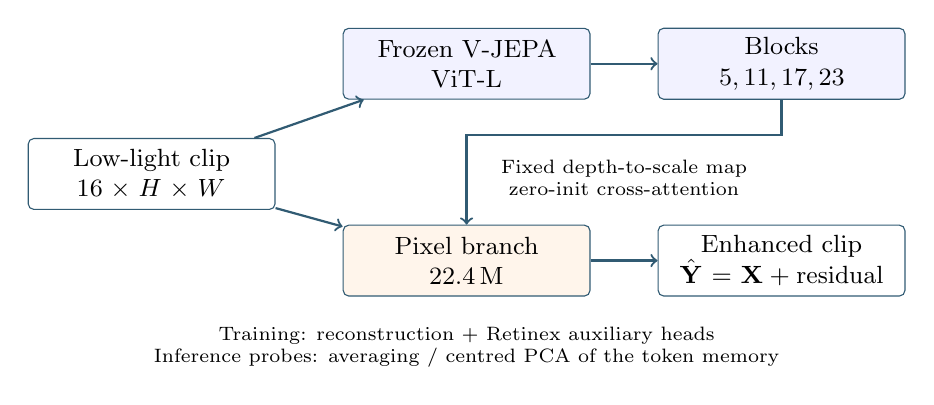
\begin{tikzpicture}[
  box/.style={draw=linkink,rounded corners=2pt,align=center,
              minimum height=9mm,text width=29mm,font=\small},
  memory/.style={box,fill=blue!5},
  train/.style={box,fill=orange!8},
  arr/.style={->,thick,draw=linkink},
  note/.style={font=\scriptsize,align=center}
]
\node[box] (input) at (0,0) {Low-light clip\\$16\times H\times W$};
\node[memory] (encoder) at (4,1.4) {Frozen V-JEPA\\ViT-L};
\node[memory] (tokens) at (8,1.4) {Blocks\\$5,11,17,23$};
\node[train] (pixel) at (4,-1.1) {Pixel branch\\$22.4$\,M};
\node[box] (output) at (8,-1.1) {Enhanced clip\\$\Yhat=\X+\mathrm{residual}$};
\node[note] (inject) at (6,-0.05) {Fixed depth-to-scale map\\zero-init cross-attention};
\draw[arr] (input) -- (encoder);
\draw[arr] (encoder) -- (tokens);
\draw[arr] (input) -- (pixel);
\draw[arr] (tokens.south) -- ++(0,-0.45) -| (pixel.north);
\draw[arr] (pixel) -- (output);
\node[note] at (4,-2.2) {Training: reconstruction + Retinex auxiliary heads\\
Inference probes: averaging / centred PCA of the token memory};
\end{tikzpicture}
}
\caption{The studied Seer-v2 model. A frozen video encoder supplies four token
fields to a small trainable pixel branch through fixed scale assignments.
Token interventions change this memory while leaving the trained branch fixed.
Auxiliary reflectance and illumination heads are used only during training.}
\label{fig:arch}
\end{figure}

\paragraph{Frozen memory.}
We use the released V-JEPA\,2.1 ViT-L checkpoint distilled from ViT-G
\citep{vjepa2}. The encoder is frozen throughout restoration training.
It receives $16$ frames resized to $256\times256$, producing
$8\times16\times16=2048$ tokens of width $1024$ at each of blocks
$\Lset=\{5,11,17,23\}$ (zero-indexed).
At spatial scales $1/2,1/4,1/8,1/16$, the pixel branch reads these four
fields respectively, with the same assignment in the decoder.
There is no learned mixture across depths.

For frame $t$, $Z_{s,t}$ contains the $256$ spatial tokens from tubelet
$\lfloor t/2\rfloor$ at the assigned depth. Encoder and decoder features at
scale $s$ read this memory through residual multi-head cross-attention,
\begin{equation}\label{eq:xattn}
F_{s,t}\leftarrow F_{s,t}+W^s_o
  \operatorname{Attn}(F_{s,t}W^s_Q,Z_{s,t}W^s_K,Z_{s,t}W^s_V).
\end{equation}
The output projection $W^s_o$ starts at zero. The default attention has no
added query--key positional correspondence; spatial grounding is a separate
intervention.

\paragraph{Objective.}
Training-only heads predict reflectance $\hat R$ and illumination $\hat L$.
The default loss is
\begin{equation}\label{eq:loss}
\mathcal L_0=
1.5\,\rho(\Yhat,\Y)+
0.15\,\rho(\hat R\odot\hat L,\Y)+
0.02\,\mathrm{TV}_{xy}(\hat L),
\end{equation}
where $\rho$ is the mean Charbonnier loss with $\epsilon=10^{-3}$ and
$\mathrm{TV}_{xy}$ is spatial total variation. Inference uses the clipped
residual prediction without exposure or colour calibration.

\subsection{Intervening on the memory}\label{sec:method:interventions}

Spatial averaging replaces each tubelet's tokens with their spatial mean;
temporal averaging replaces each spatial position with its mean over
tubelets. Both broadcast the result to the original grid, preserving the
attention tensor shapes.

For one clip and tap, write $Z\in\mathbb R^{2048\times1024}$ and let
$\mu_Z$ be its mean token. If $V_{Z,k}$ contains the top $k$ principal
directions of $Z-\mathbf1\mu_Z$, the per-clip intervention is
\begin{equation}\label{eq:cliprank}
\mathcal T^{\mathrm{clip}}_k(Z)=
\mathbf1\mu_Z+(Z-\mathbf1\mu_Z)V_{Z,k}V_{Z,k}^{\top}.
\end{equation}
This preserves a full $1024$-dimensional clip mean; only the centred token
variation is restricted to rank $k$.
The fixed intervention uses a mean $\mu_{\rm tr}$ and directions
$V_{{\rm tr},k}$ estimated separately for each tap from training clips,
\begin{equation}\label{eq:globalrank}
\mathcal T^{\mathrm{fixed}}_k(Z)=
\mathbf1\mu_{\rm tr}+
(Z-\mathbf1\mu_{\rm tr})V_{{\rm tr},k}V_{{\rm tr},k}^{\top}.
\end{equation}
The comparison changes both the mean and the basis; it does not isolate basis
adaptivity alone.
An exploratory validation control crosses the two means and the two bases
using the same reconstruction formula, alongside identity and broadcast
clip-mean controls (App.~\ref{app:meanbasis}).
The adaptive directions always come from clip-centred tokens, including when
the reconstruction uses the training-set mean.

\subsection{Testing a temporal objective}\label{sec:method:temporal}

Let $\Delta Z_t=Z_{t+1}-Z_t$ be the block-23 token difference along tubelets.
We add $0.3\mathcal L_{\Delta}$ to Eq.~\eqref{eq:loss}, with gradients through
the frozen encoder to the predicted pixels.
The relative form is
$\mathcal L_{\Delta}^{\mathrm{rel}}=
\|\Delta\Phi(\Yhat)-\Delta\Phi(\Y)\|_1/
\max(\|\Delta\Phi(\Y)\|_1,\epsilon)$.
A temporally constant prediction scores approximately one, so shrinking the
variation can reduce this objective without reconstructing the dynamics.
The cosine form instead uses
\begin{equation}\label{eq:tdcos}
\begin{aligned}
\mathcal L_{\Delta}^{\mathrm{cos}}={}&
1-\overline{\cos(\Delta\Phi(\Yhat),\Delta\Phi(\Y))}\\
&+\left|\log \frac{\max(\|\Delta\Phi(\Yhat)\|_1,\epsilon)}
                       {\max(\|\Delta\Phi(\Y)\|_1,\epsilon)}\right|,
\end{aligned}
\end{equation}
where cosine is computed per token over channels and the $\ell_1$ quantities
are mean absolute magnitudes. We record both directional
agreement and the magnitude ratio to check what the loss actually changes.

\subsection{Training}\label{sec:method:train}

All reported converged arms use a fixed $20{,}000$-step schedule.
The pixel branch starts from scratch with AdamW, learning rate
$2\times10^{-5}$, weight decay $10^{-4}$, betas $(0.9,0.99)$,
batch one and eight-step gradient accumulation.
Training uses random $256\times256$ crops of $16$-frame clips, flips,
gradient clipping at one, bf16 autocast, and gradient checkpointing.
Validation is monitored without selecting a checkpoint; the final checkpoint
is scored. The default objective contains no latent temporal term.

\section{Experiments}\label{sec:exp}

\subsection{Protocol}\label{sec:exp:protocol}

\paragraph{Data and evaluation.}
In-domain training uses the fixed SDSD~\citep{sdsd} split:
$136$ training sequences, $16$ validation sequences, and $39$ test sequences.
Scene groups are kept together when defining validation; sequences identified
as leaking between training and test were removed before this round.
For transfer we treat SDSD, BVI-RLV~\citep{bvi_rlv}, and
LOL~\citep{lol_v1,lol_v2} as three domains.
BVI-RLV has $48/16/16$ train/validation/test clips from $24/8/8$ scenes.
The LOL domain pools LOL-v1, LOL-v2-real, and LOL-v2-synthetic, with
$215$ test images in total.
Leave-one-domain-out training samples each of the two source domains with
probability $1/2$; neither source arm sees the held-out domain.

Videos use the centre $16$ frames and a $256\times256$ centre crop.
Frames are paired by sorted index rather than filename.
LOL images are evaluated at full resolution, repeated to form the encoder's
clip input; the single image prediction is scored.
PSNR-Y is computed after uint8 rounding, using the evaluator's BT.601 luma
conversion. LPIPS uses AlexNet~\citep{lpips}.
Temporal diagnostics include LPIPS between adjacent frames (tLP), reported
as the absolute gap to the target clip's value after seed-averaging within
each arm. Such diagnostics remain sensitive to
motion and are not interchangeable with perceptual reconstruction quality.

\paragraph{Decision rule.}
The main in-domain comparison has three seeds; transfer and most interventions
have two. Differences are paired by sequence after averaging within each arm
over seeds. We use $10{,}000$ sequence-bootstrap samples for $95\%$ intervals.
A claimed effect must exclude zero and have the same sign in every seed.
These intervals describe test-sequence variation conditional on the trained
models; the sign check does not replace estimating uncertainty over a larger
population of training seeds.
Unless specified otherwise, $\Delta$ means intervention minus reference,
so higher PSNR and lower LPIPS are better.

\subsection{The prior helps in domain}\label{sec:exp:control}

\begin{table}[t]
\centering\small
\setlength{\tabcolsep}{5pt}
\begin{tabular}{lcc}
\toprule
Conditioning / model & PSNR-Y $\uparrow$ & LPIPS $\downarrow$\\
\midrule
Zero tokens & \R{indomain@abs@none} & \R{indomain@abs@none@lpips}\\
Pretrained tokens & \R{indomain@abs@prior} & \R{indomain@abs@prior@lpips}\\
\midrule
Retinexformer, retrained & \R{rf@abs@psnr} & \R{rf@abs@lpips}\\
\bottomrule
\end{tabular}
\caption{SDSD test, $n=\R{indomain@n}$. Seer-v2 arms share architecture,
from-scratch recipe and the three nominal seeds. They do not share initial
pixel weights or training random draws (App.~\ref{app:stages}).
Retinexformer uses the same training split but its own architecture and
training schedule.}
\label{tab:control}
\end{table}

Pretrained conditioning improves the matched zero-token arm by
$\R{indomain@psnr}$\,dB
($\R{indomain@psnr@ci}$) and $\R{indomain@lpips}$ LPIPS
($\R{indomain@lpips@ci}$).
All three seeds agree in sign on both metrics.
The PSNR effect varies substantially across seeds, so its mean is evidence of
benefit under this protocol rather than a promise of a fixed improvement on
every run.
Because both arms start from scratch, this comparison avoids inheriting a
branch already adapted to the pretrained tokens.
The matched comparison alone does not separate the value of pretraining from
every possible alternative feature source.
The archived random control instantiated a different random encoder at
evaluation. Reusing the training seed instead yields
$\R{audit@random@psnr@b}$\,dB and
$\R{audit@random@lpips@b}$ LPIPS for that seed-zero checkpoint.
Against the corresponding pretrained seed, the differences are
$\R{audit@random@psnr}$\,dB ($\R{audit@random@psnr@ci}$) and
$\R{audit@random@lpips}$ LPIPS ($\R{audit@random@lpips@ci}$).
Only LPIPS resolves a benefit. This is a single trained random-control seed,
so its sequence interval cannot establish consistency over training seeds.

\paragraph{Comparison with a retrained restorer.}
Retinexformer~\citep{retinexformer} is retrained for $160{,}000$ steps on the
same SDSD training split.
Seer-v2's mean PSNR margin is $\R{vsrf@psnr}$\,dB
($\R{vsrf@psnr@ci}$), but its median is
$\R{vsrf@median}$\,dB and it wins only
$\R{vsrf@won}/\R{vsrf@n}$ sequences.
Its LPIPS difference is $\R{vsrf@lpips}$
($\R{vsrf@lpips@ci}$).
Neither interval excludes zero. The uneven sequence-level margin and different
model sizes preclude a claim of uniform superiority.
Our split and evaluation crop also differ from published benchmark tables,
so those absolute scores are not directly comparable.

\begin{figure*}[t]
\centering
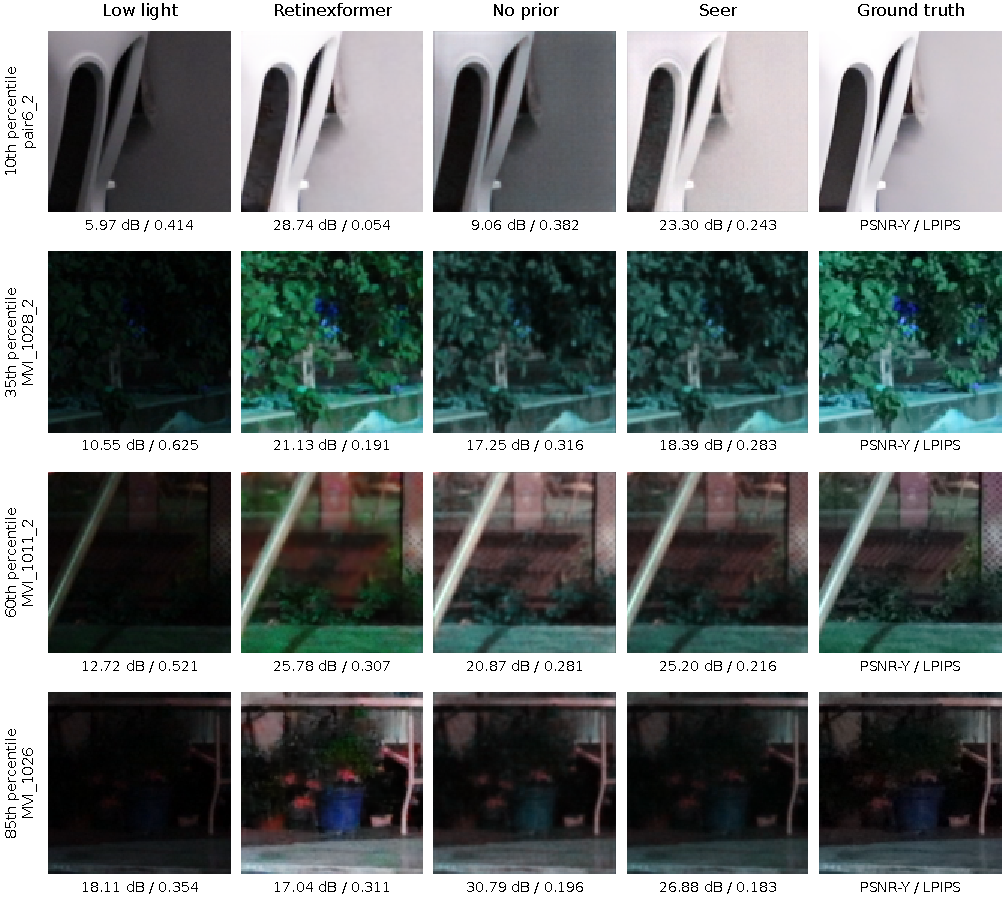
\includegraphics[width=\textwidth]{figures/fig_qualitative_cvpr.pdf}
\caption{Qualitative comparison, with columns showing input, retrained
Retinexformer, zero-token Seer-v2, pretrained Seer-v2, and ground truth.
Sequences are selected at four fixed quantiles of the sequence-level
PSNR-Y margin between the three-seed pretrained average and Retinexformer.
Displayed panel metrics score one middle frame, whereas the tables score
the full evaluation clip. Panels use pretrained and zero-token seed zero;
checkpoint, source and image hashes accompany the released figure.}
\label{fig:qualitative}
\end{figure*}

\subsection{The prior transfers under held-out-domain training}
\label{sec:exp:xdomain}

\begin{table*}[t]
\centering\small
\setlength{\tabcolsep}{8pt}
\begin{tabular}{lcll}
\toprule
Held out & $n$ & $\Delta$ PSNR-Y [95\% CI] & $\Delta$ LPIPS [95\% CI]\\
\midrule
SDSD & \R{xdom@sdsd@n} &
\R{xdom@sdsd@psnr}\ \R{xdom@sdsd@psnr@ci} &
\R{xdom@sdsd@lpips}\ \R{xdom@sdsd@lpips@ci}\\
BVI-RLV & \R{xdom@bvi@n} &
\R{xdom@bvi@psnr}\ \R{xdom@bvi@psnr@ci} &
\R{xdom@bvi@lpips}\ \R{xdom@bvi@lpips@ci}\\
LOL & \R{xdom@lol@n} &
\R{xdom@lol@psnr}\ \R{xdom@lol@psnr@ci} &
\R{xdom@lol@lpips}\ \R{xdom@lol@lpips@ci}\\
\bottomrule
\end{tabular}
\caption{Leave-one-domain-out transfer: pretrained minus zero-token
conditioning, two seeds per arm. A domain passes the registered rule when one
metric improves significantly, every seed agrees on that metric, and the other
metric has no significant degradation. SDSD and BVI-RLV pass on LPIPS; LOL
passes on PSNR-Y.}
\label{tab:xdomain}
\end{table*}

The registered transfer criterion requires improvement on at least one metric
in at least two held-out domains, without significant degradation of the other
metric. All three domains satisfy it (Table~\ref{tab:xdomain}).
The metric that improves differs: perceptual distance on SDSD and BVI-RLV,
and luminance fidelity on LOL.
This supports transfer of useful conditioning under the specified source
mixtures. It does not establish simultaneous improvement on every metric or
universal transfer to arbitrary sensors.
LOL is an image-domain test, so its improvement supplies no evidence of
temporal transfer.

\subsection{What a converged branch tolerates}\label{sec:exp:sufficiency}

\begin{table}[t]
\centering\small
\setlength{\tabcolsep}{3pt}
\begin{tabular}{lcl}
\toprule
Inference intervention & Seeds & $\Delta$ PSNR-Y [95\% CI]\\
\midrule
Per-clip centred rank 4 & \R{suff@seeds} &
\makecell[l]{\R{suff@rank4@d}\\\R{suff@rank4@ci}}\\
Spatial mean & \R{suff@seeds} &
\makecell[l]{\R{suff@spatial@d}\\\R{suff@spatial@ci}}\\
Temporal mean & \R{suff@seeds} &
\makecell[l]{\R{suff@temporal@d}\\\R{suff@temporal@ci}}\\
\midrule
Fixed rank 4 & \R{gsuff@seeds} &
\makecell[l]{\R{gsuff@global4}\\\R{gsuff@global4@ci}}\\
Fixed rank 16 & \R{gsuff@seeds} &
\makecell[l]{\R{gsuff@global16}\\\R{gsuff@global16@ci}}\\
Fixed rank 64 & \R{gsuff@seeds} &
\makecell[l]{\R{gsuff@global64}\\\R{gsuff@global64@ci}}\\
\bottomrule
\end{tabular}
\caption{Inference-only interventions on full-token-trained checkpoints,
paired with their identity controls on the same $39$ SDSD clips.
Per-clip projection retains the full clip mean; fixed projection uses the
training-set mean and basis. The two blocks have different seed counts.}
\label{tab:sufficiency}
\end{table}

Keeping four principal directions of each clip's centred tokens improves
PSNR-Y by $\R{suff@rank4@d}$\,dB
($\R{suff@rank4@ci}$), with all three seeds agreeing.
The corresponding $1024$-dimensional mean and the basis itself remain
clip-dependent. This is evidence that much of the within-clip token variation
can be removed after training; it is not a four-dimensional representation of
the whole clip.

Spatial or temporal averaging does not produce a significant PSNR change.
Their intervals are broad: the data still admit losses of roughly
$\R{suff@spatial}$\,dB and $\R{suff@temporal}$\,dB, respectively.
Absence of a detected degradation is therefore weaker than equivalence or
proof that the original field carries no useful spatial or temporal detail.

Fixed rank-4 and rank-16 replacements significantly degrade PSNR; fixed
rank-64 does not.
The contrast establishes that this fixed low-rank replacement is less
compatible with the learned branch than the per-clip replacement.
Because Eqs.~\eqref{eq:cliprank} and~\eqref{eq:globalrank} differ in both mean
and basis, that contrast cannot assign the gap solely to basis adaptivity.
Nor does it establish that the frozen encoder is impossible to replace.

\paragraph{Separating mean and basis on validation.}
An exploratory follow-up crosses both factors on all
$\R{meanval@n}$ SDSD validation sequences
($\R{meanval@scenes}$ scenes, $\R{meanval@seeds}$ existing seeds;
App.~\ref{app:meanbasis}).
Holding the clip mean fixed, adaptive rather than fixed rank-four directions
change PSNR-Y by $\R{meanval@clipvsfixed@psnr}$\,dB, with unadjusted
scene-bootstrap interval $\R{meanval@clipvsfixed@psnr@sceneci}$ and
positive effects in both seeds. Holding either basis fixed also favours the
clip mean over the training mean. This implicates both factors on validation;
it does not establish a training bottleneck or a cheaper encoder.
Rank-four projection versus identity remains inconclusive on this split.

Training-time projection addresses a different question.
The archived fixed-rank training evaluation did not restore its input
projection. Corrected evaluation applies the saved training-set mean and
rank-$64$ basis at inference as well.
Against full-token-trained seeds zero and one, its PSNR difference is
$\R{audit@grank64@psnr}$\,dB
($\R{audit@grank64@psnr@ci}$), and its LPIPS difference is
$\R{audit@grank64@lpips}$ ($\R{audit@grank64@lpips@ci}$).
The per-seed PSNR differences have opposite signs.
Neither interval resolves a difference, so the earlier significant
training-time penalty is withdrawn. These intervals also do not establish
equivalence or a faster model: the projection still follows the full encoder.

\subsection{Injection changes have mixed outcomes}
\label{sec:exp:ablation}

Restoring the saved hybrid key/value configuration also changes its archived
evaluation. Against the corresponding per-tubelet seeds zero and one,
hybrid keys change PSNR-Y by $\R{audit@hybrid@psnr}$\,dB
($\R{audit@hybrid@psnr@ci}$) and LPIPS by
$\R{audit@hybrid@lpips}$ ($\R{audit@hybrid@lpips@ci}$).
LPIPS improves in both seeds; PSNR remains unresolved.
This supports a modest perceptual benefit for this tested key/value variant.

Spatial grounding adds positional correspondence between pixel queries and
token keys. Over two seeds, its PSNR difference is
$\R{inj@spatial@psnr}$\,dB
($\R{inj@spatial@psnr@ci}$), and its LPIPS difference is
$\R{inj@spatial@lpips}$ ($\R{inj@spatial@lpips@ci}$).
Neither metric resolves an improvement at convergence.

Exposure decoupling adds a predicted global gain and a supervised exposure
objective. In its two-seed comparison, PSNR changes by
$\R{inj@edc@psnr}$\,dB ($\R{inj@edc@psnr@ci}$), while LPIPS changes by
$\R{inj@edc@lpips}$ ($\R{inj@edc@lpips@ci}$), both worse.
The spatial and exposure interventions do not justify their added structure
under this protocol. A corrected all-depth comparison is limited to one
variant seed with different training hardware (App.~\ref{app:pending});
deepest-only taps and learned gates still await verified evaluation.

\subsection{A temporal objective engages a different target}
\label{sec:exp:temporal}

The encoder is sensitive to temporal structure on this data.
The archived eight-clip probe detects a substantial block-23 token change
after shuffling under its relative token-distance measure.
This is a measurement of the encoder, separate from the restorer.

The relative temporal loss reduces the latent magnitude ratio to
$\R{h17@tdrel@mag}$ and leaves directional agreement at
$\R{h17@tdrel@cos}$.
Its LPIPS and tLP-gap changes are
$\R{h17@tdrel@lpips}$ ($\R{h17@tdrel@lpips@ci}$) and
$\R{h17@tdrel@tlp}$ ($\R{h17@tdrel@tlp@ci}$), respectively:
the loss rewards a smaller latent variation without improving the measured
reconstruction.

The cosine form restores the magnitude ratio to $\R{h17@tdcos@mag}$ and
reaches directional agreement $\R{h17@tdcos@cos}$.
Nevertheless LPIPS worsens by $\R{h17@tdcos@lpips}$
($\R{h17@tdcos@lpips@ci}$) and the tLP gap worsens by
$\R{h17@tdcos@tlp}$ ($\R{h17@tdcos@tlp@ci}$).
PSNR is unresolved:
$\R{h17@tdcos@psnr}$\,dB ($\R{h17@tdcos@psnr@ci}$).
The archived order probe for this model changes aggregate PSNR by only
$\R{ordersens}$\,dB after shuffling.
These observations distinguish matching latent temporal differences from
improving the pixel-space result; the former does not guarantee the latter.

\subsection{Why training budget belongs in the conclusion}
\label{sec:exp:budget}

The initial short-budget round and the converged round lead to different
decisions about the conditioning benefit, transfer, and temporal interventions.
Consequently, all effect estimates used above come from the fixed
$20{,}000$-step schedule, and early results are kept as exploratory records.
A conclusion about a small architectural effect requires that the reference
and intervention have both been trained long enough to make that comparison
meaningful. This is a protocol requirement demonstrated by this study, rather
than a proposed universal iteration count.

\section{Conclusion}\label{sec:conclusion}

Frozen V-JEPA conditioning benefits a matched low-light restorer in domain and
under the specified leave-one-domain-out protocol. The stronger question is
what the trained branch uses. It tolerates removal of most centred token
variation when its clip mean and a few clip-specific principal directions are
preserved; the tested fixed replacement is much less successful. An exploratory
validation control separates contributions of the clip mean and, conditional
on that mean, adaptive directions; its rank-four versus full-field comparison
remains inconclusive. These results
characterise the trained readout and do not yet provide a smaller encoder or a
validated computational compression recipe. The corrected fixed-rank
training control has an unresolved effect rather than the previously reported
penalty, while the single-seed random control resolves a perceptual benefit
without resolving a fidelity benefit.
Hybrid keys modestly improve LPIPS, spatial grounding does not resolve an improvement, exposure decoupling
degrades the result, and directly matching latent temporal changes worsens
perceptual quality and the measured tLP gap. The study supports measuring
downstream use separately from what a pretrained model can represent, and
making those measurements on converged, reproducible comparisons.


\clearpage
\phantomsection\label{after-main-text}
\section*{Reproducibility statement}
All numbers in this paper are generated by a script from per-sequence evaluation files (\texttt{tools/make\_tables.py}); the training, evaluation and ablation code, the fixed split lists, the CP calibration clips and the per-sequence results will be released. Section~\ref{sec:method} and App.~\ref{app:impl} list every architectural and optimisation hyper-parameter; App.~\ref{app:membership} lists the training-set membership of every evaluated checkpoint.

\section*{Ethics statement}
The work uses public research datasets (SDSD, BVI-RLV, LOL) and released model weights under their licences. Low-light enhancement can be used in surveillance; we do not target identification tasks.

\bibliography{seer}
\bibliographystyle{iclr2027_conference}

\clearpage
\appendix
\section{Implementation and data details}\label{app:impl}

\paragraph{Encoder.}
The frozen checkpoint is V-JEPA\,2.1 ViT-L distilled from ViT-G at
$384$ pixels. Its input is bilinearly resized to $256\times256$ and
normalised using ImageNet statistics. Tubelet size is two, patch size is
$16$, and the $24$-block encoder is read at zero-indexed blocks
$5,11,17,23$ after the corresponding hierarchical normalisation.
This produces four $2048\times1024$ fields.
The frozen encoder contributes approximately $304.7$\,M parameters in
addition to the $22.4$\,M trainable pixel branch.
Parameter count of the pixel branch alone is not an inference-cost comparison.

\paragraph{Pixel branch.}
Attention heads are $(2,4,4,8,8)$ and the feed-forward expansion is $2.66$.
The decoder mirrors the four non-bottleneck encoder scales, with skip
concatenation and a $1\times1$ reduction.
Pixel-unshuffle and pixel-shuffle operations change resolution.
The bottleneck has a residual temporal convolution followed by cross-frame
attention; other restoration blocks operate frame-wise.
Each stage applies restoration blocks, token cross-attention where enabled,
and local illumination cue injection.
Reflectance and illumination heads are convolution--SiLU--convolution--sigmoid
stacks with three and one output channels, respectively. Their outputs
contribute only to the training loss.
The residual head is a zero-initialised $3\times3$ convolution.

\paragraph{Initialisation and optimisation.}\label{app:stages}
The converged CVPR comparisons use from-scratch pixel branches, not the
warm-started stages in the earlier project snapshot.
The frozen representation is the only pretrained part of the default model.
The zero-token arm keeps the same cross-attention modules.
The arms use the same nominal seed set, but constructing the pretrained
encoder consumes random draws before the pixel branch is initialised,
whereas the zero-token arm skips that construction. Their initial pixel
weights and training random draws are therefore not shared.
The comparison controls architecture and optimisation recipe; pairing refers
to test sequences, not to identical training randomness.
All arms use the optimiser and crop recipe in Sec.~\ref{sec:method:train}
and score the final checkpoint without validation-based selection.
The converged run collection includes both Ascend 910B3 and NVIDIA A100
runs; experiment identifiers, seeds and hardware are listed in the released
manifest. The third in-domain seed was completed on different hardware, so
the seed collection does not separately estimate hardware effects.

\paragraph{Split provenance.}\label{app:membership}
SDSD-indoor contributes $46/6/14$ train/validation/test sequences and
SDSD-outdoor $90/10/25$.
Validation groups repeated passes of a scene together.
BVI-RLV contains both frame rates of each scene; its two clips per scene
stay in the same data split.
LOL-v1 has $436/49/15$ training/validation/test images,
LOL-v2-real $620/69/100$, and LOL-v2-synthetic $810/90/100$.
The frozen split files, rather than a split reconstructed at evaluation time,
define membership.
Retinexformer is retrained on these SDSD training sequences.
Results from released checkpoints trained on other splits are excluded from
the current main comparison.

\paragraph{Evaluation details.}
Inputs and targets are paired by sorted frame index, which handles SDSD
sequences with filename offsets.
The central video clip and spatial crop are fixed before inference.
Short clips and images are repeated to $16$ frames; images produce a single
scored frame.
Image sizes are padded to the branch's spatial divisor and cropped back
after inference.
Raw predictions are clipped to $[0,1]$ and rounded to uint8 for PSNR.
GT-mean rescaling and previous colour-calibration procedures are not used in
the main claims.
The registered bootstrap unit is the evaluated sequence or image.
Paired SDSD passes and BVI-RLV frame-rate clips can share a scene.
A post-hoc sensitivity analysis therefore resamples whole scene groups,
retaining sequence weights through a total-sum/total-count estimator.
The in-domain PSNR-Y and LPIPS benefits and the two video-domain transfer
LPIPS benefits retain their direction and zero-excluding intervals.
The SDSD transfer LPIPS bound is close to zero. This robustness analysis
does not replace more training seeds or eliminate other dependence.

\section{Intervention details}\label{app:interventions}

\paragraph{Principal components.}
Per-clip projection centres all $2048$ tokens at each tap, obtains the right
singular vectors of the centred matrix, and reconstructs it after retaining
$k$ directions. The full clip mean is added back.
It therefore retains substantially more than $k$ scalar values: the mean,
directions, and token-dependent coordinates all remain.
The fixed basis uses the first $60$ training-split clips in the saved order,
accumulating means and second moments separately at each tap; eigendecomposition
gives a rank-$64$ basis, truncated to the requested rank.
No target or test label is used in either projection.
The per-clip projection nevertheless depends on the test input, as intended,
whereas the fixed basis and mean do not.

\paragraph{Exploratory mean--basis control (validation only).}\label{app:meanbasis}
The historical test intervention changes both factors.
To separate them, we use the existing full-token-trained E17 seeds zero and
one on every frozen SDSD validation sequence, without retraining or checkpoint
selection. The diagnostic was chosen after the earlier results were inspected;
its six conditions and validation-only protocol were recorded in Amendment~21
before its outcomes. It is exploratory rather than a new confirmatory test.
All principal-component projections here have rank four.
The adaptive directions are computed from clip-centred tokens independently
of which mean is used in reconstruction.

\begin{table}[t]
\centering\small
\setlength{\tabcolsep}{4pt}
\begin{tabular}{lcc}
\toprule
Validation condition & PSNR-Y $\uparrow$ & LPIPS $\downarrow$\\
\midrule
Identity & \R{meanval@identity@psnr} & \R{meanval@identity@lpips}\\
Clip mean only & \R{meanval@meanonly@psnr} & \R{meanval@meanonly@lpips}\\
Clip mean, clip basis & \R{meanval@clipclip@psnr} & \R{meanval@clipclip@lpips}\\
Clip mean, fixed basis & \R{meanval@clipfixed@psnr} & \R{meanval@clipfixed@lpips}\\
Train mean, clip basis & \R{meanval@trainclip@psnr} & \R{meanval@trainclip@lpips}\\
Train mean, fixed basis & \R{meanval@trainfixed@psnr} & \R{meanval@trainfixed@lpips}\\
\bottomrule
\end{tabular}
\caption{Exploratory mean--basis diagnostic on
$\R{meanval@n}$ validation sequences from $\R{meanval@scenes}$ scenes,
averaged over $\R{meanval@seeds}$ existing checkpoints. The four crossed
conditions use rank-four directions; clip-mean-only broadcasts the mean to
every token. These are validation measurements, separate from
Table~\ref{tab:sufficiency}'s test results.}
\label{tab:meanbasis}
\end{table}

We pair differences by sequence after seed averaging and report unadjusted
$95\%$ scene-bootstrap intervals, with $10{,}000$ resamples from eight scenes;
the archive also reports sequence-bootstrap intervals and every seed effect.
At fixed clip mean, replacing the training basis with adaptive directions
changes PSNR-Y by $\R{meanval@clipvsfixed@psnr}$\,dB
($\R{meanval@clipvsfixed@psnr@sceneci}$).
At fixed adaptive basis, replacing the training mean with the clip mean
changes it by $\R{meanval@meanvsfixedmean_clipbasis@psnr}$\,dB
($\R{meanval@meanvsfixedmean_clipbasis@psnr@sceneci}$);
with the fixed basis, the corresponding change is
$\R{meanval@meanvsfixedmean_fixedbasis@psnr}$\,dB
($\R{meanval@meanvsfixedmean_fixedbasis@psnr@sceneci}$).
Every seed agrees in sign on these contrasts.
The basis contrast at the training mean remains unresolved on PSNR,
so the adaptive-basis effect is conditional on the retained mean.

Rank-four adaptive projection also improves on clip-mean-only by
$\R{meanval@rank4vsmeanonly@psnr}$\,dB
($\R{meanval@rank4vsmeanonly@psnr@sceneci}$), with both seeds positive.
Against identity, however, the change is
$\R{meanval@rank4vsidentity@psnr}$\,dB
($\R{meanval@rank4vsidentity@psnr@sceneci}$), and LPIPS effects have
opposite signs across seeds. This does not establish equivalence or a
validation improvement over the full field.
The matched contrasts support contributions from both the input-dependent
mean and basis under these interventions. They do not show that either can be
obtained cheaply, that a trained model needs only four dimensions, or that the
same representation suffices during training.

\paragraph{Interpretation of averaging.}
Spatial mean retains a separate vector for each tubelet; temporal mean retains
a separate vector for each spatial position.
Neither transformation removes the frozen encoder's computation.
An interval that crosses zero bounds the detected effect but does not establish
statistical equivalence without a predeclared equivalence margin.

\paragraph{Temporal measurements.}
The latent diagnostic reports mean cosine agreement of consecutive-tubelet
differences and their mean absolute magnitude ratio.
The relative and cosine losses are trained on two seeds each.
The cosine form's log-ratio penalty penalises both expansion and contraction.
For each sequence and arm, tLP and target tLP are averaged over the arm's
seeds, then their absolute difference is taken. Differences between these
absolute gaps are paired over sequences. Each individual seed's absolute-gap
effect is also checked for the same sign.
The order of averaging and taking the absolute value matches the released
aggregation tool. This gap uses identical frames and crops and is not a
motion-compensated error.

\section{Corrected controls and outstanding validation}\label{app:pending}

The archive contains evaluations beyond those used in the current claims.
The random-encoder control has now been rescored with CPU initialisation seed
$1234$, matching the training implementation. Its recorded initial-parameter
checksum agrees up to the float-versus-double accumulation difference logged
by the NPU runtime; this is an approximate fingerprint, not a full model hash.
The corrected JSON records reconstruction settings separately from the
historical result. Section~\ref{sec:exp:control} uses the corrected single-seed
comparison and does not retain the earlier large fidelity-attribution claim.

Corrected hybrid cross-frame keys are reported in
Sec.~\ref{sec:exp:ablation}. Restoring all-depth keys for the available
seed-two checkpoint gives $\R{audit@alllayers@psnr@a}$\,dB, replacing the
archived, incorrectly configured $21.568$\,dB result. Against the corresponding
full-token default seed, its differences are
$\R{audit@alllayers@psnr}$\,dB ($\R{audit@alllayers@psnr@ci}$) and
$\R{audit@alllayers@lpips}$ LPIPS ($\R{audit@alllayers@lpips@ci}$).
Both intervals include zero. The variant was trained on Ascend and the
reference on A100, with only one available variant seed; this conditional
comparison cannot establish a general architectural effect. Its temporal
diagnostics also show tradeoffs, detailed in the audit record.
Deepest-only taps and learned gates still require the actual trained
configuration and weights before their archived differences can support
architectural conclusions.
The fixed-rank-$64$ training control has been reevaluated with its saved
projection. Its current comparison uses the same two baseline seed numbers;
the old three-baseline-seed comparison is preserved in the audit record.
Neither comparison resolves a training-time penalty after correction.
It still does not establish a computational compression result.

H20/E28, training from scratch with per-clip centred rank-four tokens, remains
unfinished: no verified final evaluation is available.
It is neither a positive nor a negative result.
The proposed small-network distillation experiment was cancelled by its
registered screening rule and was not run; its cancellation supplies no
evidence that another encoder or distillation procedure cannot work.
Some baseline temporal diagnostics were not included in the original archive.
Claims requiring those missing measurements are withheld until they are
reproduced under the same protocol. The qualitative panels have been
regenerated with checkpoint, source and output hashes.

\section{Scope of the conclusions}\label{app:scope}

The main conclusions concern one frozen encoder, one restoration family,
and the specified data splits.
Few seeds limit inference about training variability, and sequence bootstraps
do not replace additional independent runs.
SDSD includes low-motion material, while the LOL test contains still images.
A video encoder's temporal sensitivity and a readout's weak order sensitivity
therefore do not prove that temporal representations are irrelevant to other
video-restoration tasks.
The tested low-rank replacements describe the behaviour of existing
checkpoints. The exploratory validation control separates mean and basis
effects under those replacements; future work must separately test efficient
encoders and training with the restricted representation.

\end{document}
